% !TEX TS-program = XeLaTeX
% use the following command:
% all document files must be coded in UTF-8
\documentclass[portuguese]{textolivre}
% build HTML with: make4ht -e build.lua -c textolivre.cfg -x -u article "fn-in,svg,pic-align"

\journalname{Texto Livre}
\thevolume{15}
%\thenumber{1} % old template
\theyear{2022}
\receiveddate{\DTMdisplaydate{2022}{3}{9}{-1}} % YYYY MM DD
\accepteddate{\DTMdisplaydate{2022}{4}{4}{-1}}
\publisheddate{\DTMdisplaydate{2022}{5}{27}{-1}}
\corrauthor{Daniel Gomes da Cunha}
\articledoi{10.35699/1983-3652.2022.38695}
%\articleid{NNNN} % if the article ID is not the last 5 numbers of its DOI, provide it using \articleid{} commmand 
% list of available sesscions in the journal: articles, dossier, reports, essays, reviews, interviews, editorial
\articlesessionname{articles}
\runningauthor{Cunha e Silva} 
%\editorname{Leonardo Araújo} % old template
\sectioneditorname{Daniervelin Pereira}
\layouteditorname{Leonado Araújo}

\title{\textit{Corpus} de legendas de \textit{animes} (CorLeAni)}
\othertitle{\textit{Anime} subtitles \textit{corpus} (CorLeAni)}
% if there is a third language title, add here:
%\othertitle{Artikelvorlage zur Einreichung beim Texto Livre Journal}

\author[1,2]{Daniel Gomes da Cunha \orcid{0000-0001-6075-3950} \thanks{Email: \url{dng20@hotmail.com}}}
\author[3]{Janailton Mick Vitor da Silva \orcid{0000-0002-5137-5473} \thanks{Email: \url{janailtonm@gmail.com}}}
\affil[1]{Centro de Ensino Unificado de Brasília, Brasília, DF, Brasil.}
\affil[2]{Faculdade de Tecnologia e Ciências Sociais Aplicadas, Brasília, DF, Brasil.}
\affil[3]{Instituto Federal de Brasília - Campus Ceilândia, Brasília, DF, Brasil.}

\addbibresource{article.bib}
% use biber instead of bibtex
% $ biber article

% used to create dummy text for the template file
\definecolor{dark-gray}{gray}{0.35} % color used to display dummy texts
\usepackage{lipsum}
\SetLipsumParListSurrounders{\colorlet{oldcolor}{.}\color{dark-gray}}{\color{oldcolor}}

% used here only to provide the XeLaTeX and BibTeX logos
\usepackage{hologo}

% if you use multirows in a table, include the multirow package
\usepackage{multirow}

% provides sidewaysfigure environment
\usepackage{rotating}

% CUSTOM EPIGRAPH - BEGIN 
%%% https://tex.stackexchange.com/questions/193178/specific-epigraph-style
\usepackage{epigraph}
\renewcommand\textflush{flushright}
\makeatletter
\newlength\epitextskip
\pretocmd{\@epitext}{\em}{}{}
\apptocmd{\@epitext}{\em}{}{}
\patchcmd{\epigraph}{\@epitext{#1}\\}{\@epitext{#1}\\[\epitextskip]}{}{}
\makeatother
\setlength\epigraphrule{0pt}
\setlength\epitextskip{0.5ex}
\setlength\epigraphwidth{.7\textwidth}
% CUSTOM EPIGRAPH - END

% LANGUAGE - BEGIN
% ARABIC
% for languages that use special fonts, you must provide the typeface that will be used
% \setotherlanguage{arabic}
% \newfontfamily\arabicfont[Script=Arabic]{Amiri}
% \newfontfamily\arabicfontsf[Script=Arabic]{Amiri}
% \newfontfamily\arabicfonttt[Script=Arabic]{Amiri}
%
% in the article, to add arabic text use: \textlang{arabic}{ ... }
%
% RUSSIAN
% for russian text we also need to define fonts with support for Cyrillic script
% \usepackage{fontspec}
% \setotherlanguage{russian}
% \newfontfamily\cyrillicfont{Times New Roman}
% \newfontfamily\cyrillicfontsf{Times New Roman}[Script=Cyrillic]
% \newfontfamily\cyrillicfonttt{Times New Roman}[Script=Cyrillic]
%
% in the text use \begin{russian} ... \end{russian}
% LANGUAGE - END

% EMOJIS - BEGIN
% to use emoticons in your manuscript
% https://stackoverflow.com/questions/190145/how-to-insert-emoticons-in-latex/57076064
% using font Symbola, which has full support
% the font may be downloaded at:
% https://dn-works.com/ufas/
% add to preamble:
% \newfontfamily\Symbola{Symbola}
% in the text use:
% {\Symbola }
% EMOJIS - END

% LABEL REFERENCE TO DESCRIPTIVE LIST - BEGIN
% reference itens in a descriptive list using their labels instead of numbers
% insert the code below in the preambule:
%\makeatletter
%\let\orgdescriptionlabel\descriptionlabel
%\renewcommand*{\descriptionlabel}[1]{%
%  \let\orglabel\label
%  \let\label\@gobble
%  \phantomsection
%  \edef\@currentlabel{#1\unskip}%
%  \let\label\orglabel
%  \orgdescriptionlabel{#1}%
%}
%\makeatother
%
% in your document, use as illustraded here:
%\begin{description}
%  \item[first\label{itm1}] this is only an example;
%  % ...  add more items
%\end{description}
% LABEL REFERENCE TO DESCRIPTIVE LIST - END


% add line numbers for submission
%\usepackage{lineno}
%\linenumbers

% new column type 
\newcolumntype{S}{>{\hsize=.5\hsize}X}

\usepackage{calc}
\newlength\myheight
\newlength\mydepth
\settototalheight\myheight{Xygp}
\settodepth\mydepth{Xygp}
\setlength\fboxsep{0pt}
\newcommand*\inlinegraphics[1]{%
  \settototalheight\myheight{Xygp}%
  \settodepth\mydepth{Xygp}%
  \raisebox{-\mydepth}{\includegraphics[height=\myheight]{#1}}%
}

\usepackage[section]{placeins}
\makeatletter
\AtBeginDocument{%
  \expandafter\renewcommand\expandafter\subsection\expandafter{%
    \expandafter\@fb@secFB\subsection
  }%
}
\makeatother

\begin{document}
\maketitle

\begin{polyabstract}
\begin{abstract}
Reportamos, neste artigo, o processo de compilação de um \textit{corpus} formado por legendas de \textit{animes} em português brasileiro, aqui denominado Corpus de Legendas de Animes (CorLeAni). O CorLeAni, atualmente com cerca de 1 milhão de palavras, foi compilado seguindo o suporte teórico-metodológico dos Estudos da Tradução Baseados em Corpus. A compilação deu-se ao longo de dois Projetos de Pesquisa de Iniciação Científica de Ensino Médio (PIBIC-EM), 2019-2020 e 2020-2021, com bolsa do Instituto Federal Goiano-\textit{Campus} Campos Belos. Reconhecendo que as \textit{fansubs} apresentam um grande potencial para discussões e estudos no âmbito audiovisual, disponibilizamos o CorLeAni de forma gratuita, podendo ser utilizado em futuras pesquisas com focos linguístico e tradutório.

\keywords{\textit{Anime} \sep \textit{Corpus} \sep \textit{Fansubber} \sep \textit{Fansubs} \sep Legendagem}
\end{abstract}

\begin{english}
\begin{abstract}
We report, in this article, the process of compiling a corpus consisting of \textit{anime} subtitles in Brazilian Portuguese, hereby named Anime Subtitles Corpus (CorLeAni). The corpus, currently with almost 1 million words, has been compiled following the theoretical-methodological support of Corpus-Based Translation Studies. The compilation took place over two Projects of Scientific Initiation of High School (PIBIC-EM), 2019-2020 and 2020-2021, with a grant from the Instituto Federal Goiano-Campus Campos Belos. Recognizing that fansubs have great potential for discussions and studies in the audiovisual field, we have made CorLeAni available for free so it can be used in future linguistic and translation research.

\keywords{\textit{Anime} \sep \textit{Corpus} \sep Fansubber \sep Fansubs \sep Subtitling}
\end{abstract}
\end{english}
% if there is another abstract, insert it here using the same scheme
\end{polyabstract}

\section{Introdução}\label{sec-intro}
Em Díaz Cintas (2013), o autor destaca que vivemos na era da audiovisualização, onde testemunhamos várias manifestações tradutórias em mídias diversas, como a legendagem, dublagem, \textit{voice-over}, narração, audiodescrição, entre outras. Em prosseguimento as suas reflexões, \textcite{diaz_cintas_taking_2015} reconhecem, ademais, a Tradução Audiovisual, área que abrange essas e outras manifestações tradutórias, como uma das áreas que mais crescem dentro dos Estudos da Tradução, principalmente por se associar com tecnologias que estão em rápida e constante evolução.

Nesse contexto da Tradução Audiovisual, sobretudo da legendagem, compreendemos as legendas como sendo textos escritos, advindos de textos orais, de sons e textos multissemióticos, bem como imagens, símbolos, inscrições imagéticas e outros \cite{diaz-cintas_audiovisual_2007}. Partindo dessa compreensão, neste artigo, reportamos o processo de compilação de um \textit{corpus} utilizando legendas produzidas para \textit{animes}, aqui denominado \textit{Corpus} de Legendas de Animes (CorLeAni). Tendo em vista a necessidade de ampliação de análises linguísticas e de fenômenos tradutórios dentro dos Estudos da Tradução Baseados em Corpus (ETBC), desenvolvemos dois Projetos de Pesquisa de Iniciação Científica de Ensino Médio (PIBIC-EM), 2019-2020 e 2020-2021, com bolsa do Instituto Federal Goiano-\textit{Campus} Campos Belos. Sendo desenvolvidas pelo primeiro autor e orientadas pelo segundo autor deste artigo, a primeira pesquisa (2019-2020) objetivou o início da compilação do \textit{corpus}, enquanto a segunda (2020-2021) buscou a expansão do CorLeAni já criado anteriormente, a partir da inserção de novos textos e a consolidação da metodologia empregada nesse processo. Em ambos os casos, fomos motivados particularmente pela crescente demanda para se entender o processo de criação de legendas de \textit{animes}, bem como o modo no qual a língua portuguesa e as outras linguagens são empregadas nessas legendas. Para tanto, foi feita uma compilação criteriosa do \textit{corpus}, conforme discutiremos mais adiante. Ademais, buscamos disponibilizar\footnote{Conforme \textit{site} a seguir: \url{http://corleani.epizy.com}} o CorLeAni em sua versão atual para a comunidade acadêmica, a fim de que possa ser utilizado em futuras pesquisas e estudos voltados ao uso da língua portuguesa traduzida no contexto dos \textit{animes}.

Feita a exposição dos percursos realizados pela pesquisa, para este artigo trazemos os resultados de ambos os projetos PIBIC-EM. Em primeiro lugar, apresentaremos os conceitos teóricos que iluminaram a compreensão do tema, seguido do passo a passo metodológico empreendido na compilação do CorLeAni. Por fim, lançaremos mão dos resultados gerais quantitativos obtidos por meio da inserção dos arquivos de legendas no \textit{WordSmith Tools©}, versão 7. No processo de compilação do \textit{corpus}, salientamos que utilizamos, além de programas pagos, alguns programas gratuitos, como \textit{Aegisub} e \textit{Subtitle Edit}, conforme apresentamos na \Cref{sec-conduta} deste texto.

\section{Fundamentando as pesquisas: conceitos sobre legendagem, \textit{fansubs}, \textit{animes} e \textit{corpus}}\label{sec-normas}
\textcite{diaz-cintas_audiovisual_2007} entendem a legendagem como um conceito que pode ser entendido como uma prática tradutória, em que é apresentado um texto escrito geralmente na parte inferior da tela e visa relatar um diálogo original entre locutores. Além disso, é possível traduzir, nessas legendas, elementos discursivos que aparecem na imagem, tais como letras, inscrições, cartazes e informações presentes na trilha sonora, como é o caso de músicas e \textit{voices off}.

Nos dias de hoje, dispomos das chamadas \textit{fansubs}, que são as legendas produzidas por fãs e que também são conhecidas pelo termo ‘legendagem amadora’ \cite{bogucki_amateur_2009}. \textcite[p. 1]{diaz-cintas_fansubs:_2006} entendem as \textit{fansubs} como uma versão legendada e traduzida por fãs de um \textit{anime} japonês, e defendem que “não seria exagero afirmar que as \textit{fansubs} são a manifestação mais importante da tradução de legendas feita por fãs”\footnote{“\textit{It would be no exaggeration to state that fansubs are nowadays the most important manifestation of fan translation} [...]” \cite[p. 1, tradução nossa]{diaz-cintas_fansubs:_2006}. Neste artigo, optamos por realizar nossa própria tradução de trechos dos artigos em inglês para o português brasileiro. Especialmente para esse texto de \textcite{diaz-cintas_fansubs:_2006}, ressaltamos a publicação recente de uma versão traduzida para o português brasileiro, conforme \textcite{diaz_cintas_fansubs:_2022}.}. Trata-se de uma prática tradutória que tem o intuito de fornecer materiais legendados gratuitamente e difundi-los entre públicos de diferentes comunidades linguísticas \cite{bogucki_amateur_2009}.

De acordo com \textcite{ferrer_simo_fansubs_2005}, há, nas \textit{fansubs}, algumas características que as tornam específicas, tal como as notas e os comentários do tradutor. São ferramentas que geralmente explicam algumas tradições, celebrações e lugares. Além disso, há o uso de fontes de texto para diferenciar os atores e o uso de legendas karaokê nas músicas de abertura e encerramento, bem como outras características. 

As \textit{fansubs} foram originalmente pensadas para produção de legendas inclusive como forma de divulgar a cultura \textit{pop} japonesa \cite{diaz-cintas_fansubs:_2006}. É importante chamar a atenção para o termo ‘cultura \textit{pop} japonesa’, que engloba mensagens e imagens criadas no Japão, servindo como poderosos assimiladores de sentidos daquele contexto cultural. Atualmente, aspectos da cultura \textit{pop} japonesa se encontram espalhados pelo mundo a partir das novas tecnologias de informação e novas mídias \apud{sato2005}{pereira_cultura_2017}. Destacam-se a sua presença a partir dos mangás (histórias em quadrinhos japoneses), dos \textit{animes} e dos demais produtos comerciais que propagam tais características culturais como parte de si.

O caso do Brasil traz especificidades que chamam a atenção. Isso porque “[n]o Brasil, no entanto, muito antes d[e o] mundo ‘descobrir’ os mangás, estes já eram fartamente lidos pela comunidade dos descendentes de japoneses.” \cite[p. 8]{luyten_manga_2014}. Por se preocuparem com a manutenção do idioma e com o aprendizado de novos termos, os japoneses realizavam importações de mangás (e, posteriormente, de animes e filmes), para que eles e seus filhos continuassem tendo contato com a cultura. Assume-se, portanto, que tivemos uma grande contribuição das comunidades nipônicas na difusão dessa cultura. 

O \textit{pop} japonês se misturou com outros elementos de diversas origens, e, apesar de atrair um público muito específico, já não é mais algo tão estranho à cultura urbana brasileira \cite{neto_mangas_2017}. Para demonstrar o quão incluído o \textit{pop} japonês está na cultura urbana brasileira, \textcite{neto_mangas_2017} afirma que ocorre, por todo o Brasil, uma quantidade relevante de eventos de \textit{animes}, também chamados de ‘animencontros’. O autor ressalta que esses eventos não se limitam aos animes, abordando outros elementos da cultura \textit{pop}, oriundos inclusive de outras origens geográficas. De todo modo, quem normalmente frequenta esses ambientes são pessoas que compartilham um gosto por \textit{animes} e por mangás.

Com os interesses de entender não somente a legendagem, mas também as legendas de \textit{animes} que resultam desse processo, assumimos o conceito de corpus enquanto uma coleção de textos em formato eletrônico e que são passíveis de passarem por análises automáticas ou semiautomáticas \cite{baker_corpus-based_1996}. Tais textos podem servir como pano de fundo para serem realizadas avaliações sobre uma determinada língua, com o auxílio da Linguística de Corpus (LC). Respaldando-nos em \textcite{mcenery_corpus_2001}, sublinhamos que a LC é a área da linguística que se ocupa em estudar o lado empírico da língua, ou seja, aquilo que é, de fato, produzido por falantes, a partir da observação de dados naturais que estão contidos em um \textit{corpus}. \textcite{sardinha_linguistica_2004} orienta que a compilação de um \textit{corpus} precisa seguir alguns pré-requisitos básicos, como, por exemplo, a questão da autenticidade, escolha criteriosa e representatividade dos textos. Desse modo, a junção dos conhecimentos da LC, dos ETBC e da tradução audiovisual para o estudo dos \textit{animes} foi  extremamente frutífera para o trabalho realizado durante os dois projetos de iniciação científica, conforme prosseguimos mais detalhadamente no tópico abaixo.

\section{Passos metodológicos para criação do CorLeAni}\label{sec-conduta}
Os pressupostos metodológicos que orientaram o desenvolvimento das pesquisas PIBIC-EM 2019-2020 e 2020-2021 seguiram o paradigma interpretativista, a metodologia descritiva e a tipologia quanti-qualitativa \cite{moreira_metodologia_2008}. Além disso, afiliamo-nos aos conhecimentos teórico-metodológicos dos ETBC \cite{baker_corpora_1995,baker_corpus-based_1996,camargo_metodologia_2007}, especialmente por meio da utilização das ferramentas \textit{WordList} e \textit{Concord} do programa \textit{WordSmith Tools©}, versão 7.0, para compilar o CorLeAni com legendas, em língua portuguesa traduzida, feitas por fãs brasileiros (\textit{fansubbers}).


\subsection{Seleção dos \textit{animes} e obtenção das legendas \textit{fansubs}}\label{sec-fmt-manuscrito}
Com base no que foi desenvolvido na pesquisa PIBIC-EM 2019-2020, decidimos manter e empregar, como critério de seleção dos \textit{animes} em ambos os projetos, as 25 maiores notas de avaliações, que variam em um espectro que vai de 0 a 10. As notas foram dadas por fãs aos \textit{animes} da temporada de primavera de 2020 e retiradas no \textit{site} \textit{MyAnimeList}\footnote{Endereço do \textit{site}: \url{https://myanimelist.net/}. Acesso em: 14 Abr. 2022.}. Em sequência, utilizamos as informações do \textit{site} \textit{InfoAnime}\footnote{Endereço do \textit{site}: \url{https://www.infoanime.com.br/}. Acesso em: 14 Abr. 2022.} para buscar os grupos de \textit{fansubbers} que haviam legendado os \textit{animes} que foram criteriosamente selecionados. Nos dois \textit{sites} apropriamo-nos dos seguintes dados: a avaliação dos fãs, no \textit{site} \textit{MyAnimeList}; os nomes dos grupos \textit{fansubbers}, no \textit{site} \textit{InfoAnime}; e também a quantidade de episódios legendados pelos \textit{fansubbers}. A partir dos dados coletados, conseguimos elaborar a \Cref{tbl1} e a \Cref{tbl2}, buscando relacionar algumas dessas informações sobre os \textit{animes} que compõem o CorLeAni. 

\begin{table}[htbp]
\caption{Tabela de \textit{animes} que compõem o CorLeAni (PIBIC-EM 2019-2020).}
\label{tbl1}
\centering
\begin{tabularx}{\linewidth}{SSXSX}
\toprule
\textbf{Classificação} & \textbf{Pontuação} & \textbf{Animes} & \textbf{Episódios} & \textit{\textbf{Fansubbers}} \\ 
\midrule
1. & 9.08 & Shingeki no Kyojin parte 2 temp 3 & 10 & Kyoshiro fansub
\\ 
2.  & 8.95 & Kimetsu no Yaiba & 26 & Aenianos
\\
3.  & 8.33 & Fruits Basket  & 25 & Aenianos
\\
4.  & 8.08 & Carole \& Tuesday & 24 & Infinite
\\
5.  & 7.79 & Kono Oto Tomare! & 13 & Infinite/Punch
\\
6.  & 7.68 & Sarazanmai & 11 & Aenianos
\\
7.  & 7.61 & Isekai Quartet & 12 & Eternal Animes
\\
8.  & 7.52 & One Punch Man & 12 & Eternal Animes
\\
9.  & 7.44 & Sewayaki Kitsune no Senko-san & 12 & ECN
\\
10.  & 7.42 & Bokutachi wa Benkyou ga Dekinai & 13 & Infinite
\\    
11.  & 6.96 & Midara na Ao-chan wa Benkyou ga Dekinai & 12 & Infinite
\\
12.  & 6.76 & Kenja no Mago & 12 & Eternal Animes
\\
\bottomrule
\end{tabularx}
\source{Elaboração nossa.}
\end{table}

\begin{table}[htbp]
\caption{Tabela de \textit{animes} que compõem o CorLeAni (PIBIC-EM 2020-2021).}
\label{tbl2}
\centering
\begin{tabularx}{\linewidth}{SSXSX}
\toprule
\textbf{Classificação} & \textbf{Pontuação} & \textbf{Nome} & \textbf{Episódios} & \textit{\textbf{Fansubbers}} \\ 
\midrule
1. & 8.80 & Kaguya-sama wa Kokurasetai?: Tensai-tachi no Renai Zunousen & 12 & Boteco/Fênix Sub
\\ 
2.  & 8.19 & Honzuki no Gekokujou: Shisho ni Naru Tame ni wa Shudan wo... & 12 & Boteco
\\
3.  & 8.04 & Kakushigoto & 12 & Moshi Moshi
\\
4.  & 7.77 & Kami no Tou & 13 & Kyoshiro/TDM
\\
5.  & 7.63 & Fugou Keiji: Balance:Unlimited  (Detetive milionario- traduzido) & 11 & Seoltang
\\
6.  & 7.52 & Otome Game no Hametsu Flag shika Nai Akuyaku Reijou ni...
& 12 & Kawaii Otome
\\
7.  & 7.37 & Shokugeki no Souma: Gou no Sara & 13 & Boteco
\\
8.  & 7.36 & Appare-Ranman! & 13 & Elite Fansub
\\
9.  & 7.09 & Princess Connect! Re:Dive & 13 & Illuminati/Shakai
\\
10.  & 6.41 & Komatta Jiisan & 13 & Isekai
\\
\bottomrule
\end{tabularx}
\source{Elaboração nossa.}
\end{table}

Compartilhamos aqui, ademais, os \textit{sites} oficiais\footnote{Aenianos: \url{https://www.aenianos.org/}. Acesso em: 20 fev. 2020.
ECN: \url{http://ecn.fansubs.com.br/}. Acesso em: 20 fev. 2020.
Eternal Animes: \url{https://eternalanimes.org/}. Acesso em: 20 fev. 2020.
Infinite: \url{https://infinitefansub.com/}. Acesso em: 20 fev. 2020.
Kyoshiro fansub: \url{https://www.kyoshirofansub.com/}. Acesso em: 20 fev. 2020.
Kirinashi: \url{https://kirinashi.fansubs.com.br/}. Acesso em: 20 fev. 2020.} em que se encontravam divulgados os \textit{animes} legendados para o público, com ênfase nos \textit{animes} cujos arquivos de mídia poderiam ser baixados. Outro caso que nos possibilitou o download envolveu dois grupos de \textit{fansubbers}, \textit{Seoltang}\footnote{Endereço do \textit{site}: \url{https://seoltangs.blogspot.com/}. Acesso em: 12 fev. 2021.} e \textit{Illuminati}\footnote{Endereço do \textit{site}: \url{https://illuminatisubsbr.wordpress.com/}. Acesso em: 12 fev. 2021.}. Eles oferecem a possibilidade de fazer o download das legendas do \textit{anime} em si, em vez de somente disponibilizarem um \textit{link} para baixar o episódio.

Verificamos ainda a possibilidade de extrair as legendas disponibilizadas nos episódios utilizando os programas de legendagem \textit{Subtitle Edit}\footnote{Endereço oficial do \textit{site}: \url{http://www.nikse.dk/subtitleedit}. Acesso em: 20 fev. 2020.} (versão 3.5.10) e/ou \textit{Aegisub}\footnote{Endereço oficial do \textit{site}: \url{http://www.aegisub.org/}. Acesso em: 20 fev. 2020.} (versão 3.2.2). Observamos, logo de início, a existência de \textit{animes} que foram traduzidos pelos \textit{fansubbers}, mesmo estando eles veiculados oficialmente na \textit{Crunchyroll}\footnote{O \textit{Crunchyroll} consiste em um \textit{site} de \textit{streaming} dedicado a \textit{animes} e à cultura asiática de um modo geral, que compra direitos de transmissão de \textit{animes}, contribuindo para o financiamento de algumas obras, ajudando, assim, a fomentar o crescimento desse mercado. Endereço oficial do \textit{site}: \url{https://www.crunchyroll.com/pt-br}. Acesso em: 20 fev. 2020.}. 

Como descrito nos tópicos abaixo, realizamos duas ações que nos ajudaram a obter o nosso material para compilação do \textit{corpus}.

\subsubsection{Contato com o grupo de \textit{fansubbers}}\label{sec-formato}
Como percurso para coleta de dados, fizemos levantamento prévio dos contatos dos \textit{fansubbers}, no intuito de criar um canal de comunicação que nos permitisse solicitar as legendas a cada grupo diretamente, especialmente através do Facebook e de \textit{e-mails}.  O procedimento parecia o mais adequado no primeiro momento, pois otimizaria o tempo da pesquisa. No entanto, a abordagem não foi tão efetiva, uma vez que, ora os grupos não respondiam ao nosso contato, ora o material disponibilizado era insuficiente (falta de episódios ou a inclusão de séries que não atendiam ao nosso critério de seleção). 

 Dentre os cinco grupos de \textit{fansubbers} que entraram nos critérios de seleção, conseguimos resultados satisfatórios apenas com um grupo, a \textit{Eternal Animes}. Para esse caso, angariamos um total de 36 arquivos de legendas para três diferentes séries de \textit{anime}. Todavia, para os outros 4 grupos, tivemos que recorrer ao que se tornou a melhor estratégia para obter os episódios: o \textit{download} individual das obras, conforme descrito no subitem abaixo. No PIBIC-EM 2020-2021, procedemos apenas com o \textit{download} direto das legendas, e não pelo contato com os \textit{fansubbers}, dada a experiência adquirida com o insucesso observado no projeto anterior em relação a esse aspecto.

\subsubsection{\textit{Download} de arquivos de mídia}\label{sec-modelo}
Utilizando-nos de meios disponibilizados nos \textit{sites} oficiais dos \textit{fansubbers}, realizamos o \textit{download} dos arquivos de mídia dos \textit{animes}. No geral, esses arquivos estavam disponibilizados no formato .MKV, no serviço de armazenamento de arquivos disponibilizado pela \textit{Google} para seus usuários, o \textit{Google Drive}. Em virtude de os arquivos baixados estarem no formato .MKV, realizamos um processo de extração perpassado no subitem a seguir.

\subsubsection{Processo de extração de legendas}\label{sec-organizacao}
Podemos verificar, na imagem a seguir (\Cref{fig01}), a maneira na qual a legenda aparece no arquivo de vídeo, em uma cena do primeiro episódio do \textit{anime Sewayaki Kitsune no Senko-san}, legendado pela \textit{Infinite fansub}. Essa cena gira em torno do protagonista dessa comédia romântica, que retorna a sua residência após mais um dia exaustivo do trabalho em uma empresa exploradora, quando é surpreendido por um espírito de raposa divina. 

\begin{figure}[h!]
 \centering
 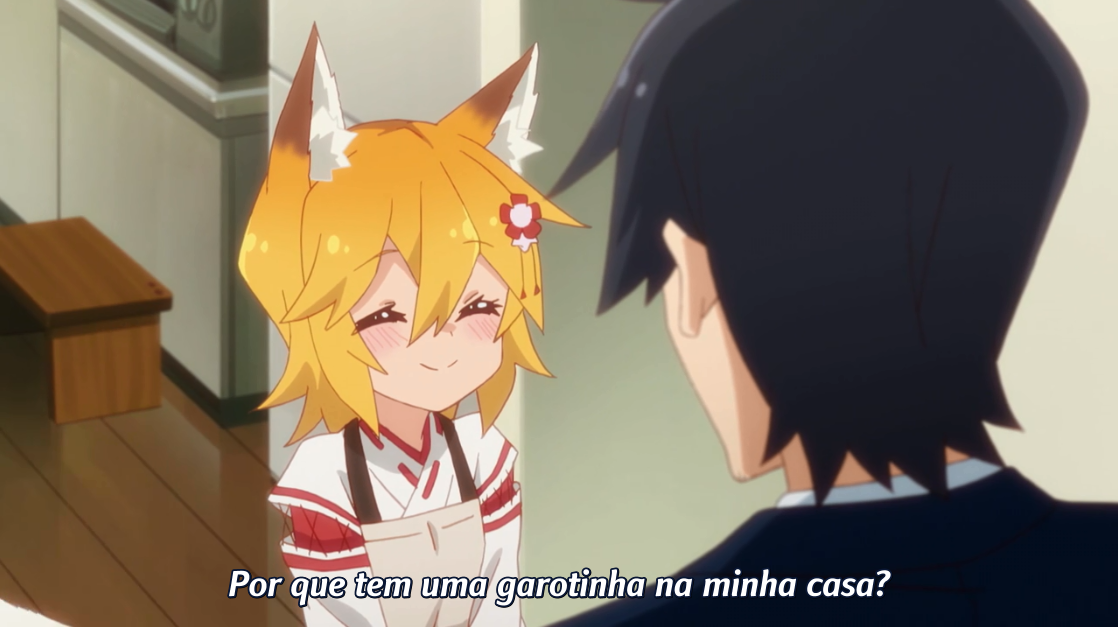
\includegraphics[width=0.85\textwidth]{Fig1.png}
 \caption{Cena de um \textit{anime} baixado: \textit{Sewayaki Kitsune no Senko-san}.}
 \label{fig01}
 \source{Elaboração nossa.}
\end{figure}

Após realizarmos o \textit{download} individual pelos meios disponibilizados pelos \textit{fansubbers}, foi feita a extração das legendas utilizando o aplicativo \textit{Subtitle Edit}. As imagens a seguir retratam a organização do material baixado no computador (\Cref{fig02}), o manuseio do programa \textit{Subtitle Edit} e o passo a passo da extração das legendas nesse programa (\Cref{fig03,fig04,fig05,fig06,fig07}). Por fim, temos o resultado do processo de extração (\Cref{fig08}). Para o caso das duas obras legendadas pela \textit{Seoltang} e pela \textit{Illuminati}, preferimos não realizar o processo de \textit{download} e extração. Optamos, nesse caso, pelo \textit{download} das legendas a partir dos \textit{links} disponibilizados por estes grupos, o que otimizou nosso tempo.

\begin{figure}[htbp]
 \centering
 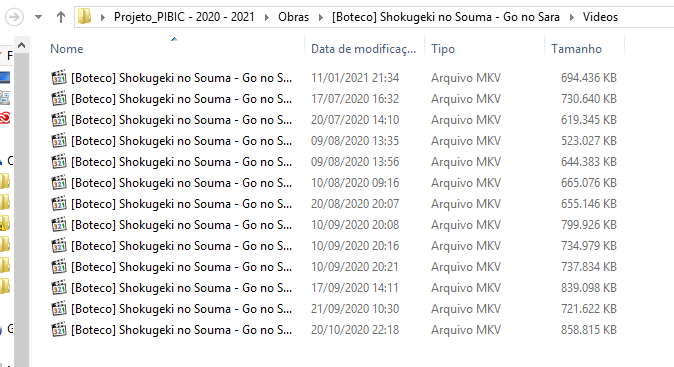
\includegraphics[width=0.85\textwidth]{Fig2.png}
 \caption{Lista de episódios do \textit{anime}: ‘\textit{Shokugeki no Souma - Go no Sara}’ após \textit{download}.}
 \label{fig02}
 \source{Elaboração nossa.}
\end{figure}

\begin{figure}[htbp]
 \centering
 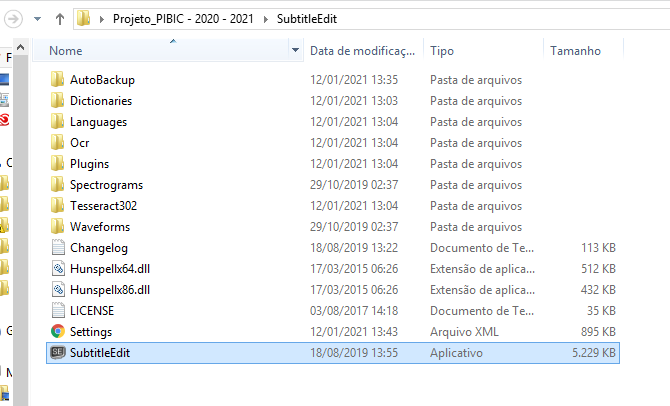
\includegraphics[width=0.85\textwidth]{Fig3.png}
 \caption{Pasta do \textit{Subtitle Edit} nos arquivos pessoais da pesquisa.}
 \label{fig03}
 \source{Elaboração nossa.}
\end{figure}

\begin{figure}[htbp]
 \centering
 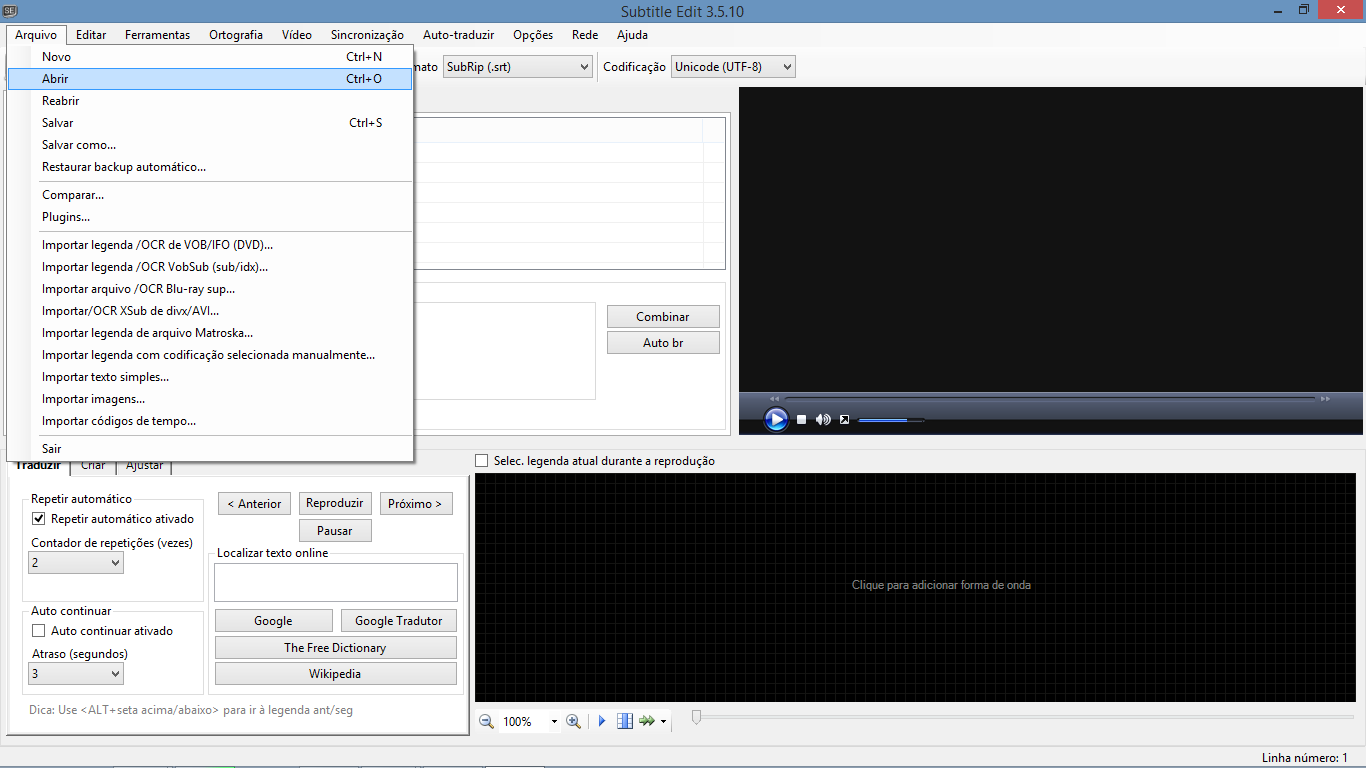
\includegraphics[width=0.85\textwidth]{Fig4.png}
 \caption{Interface inicial do programa \textit{Subtitle Edit}.}
 \label{fig04}
 \source{Elaboração nossa.}
\end{figure}

\begin{figure}[htbp]
 \centering
 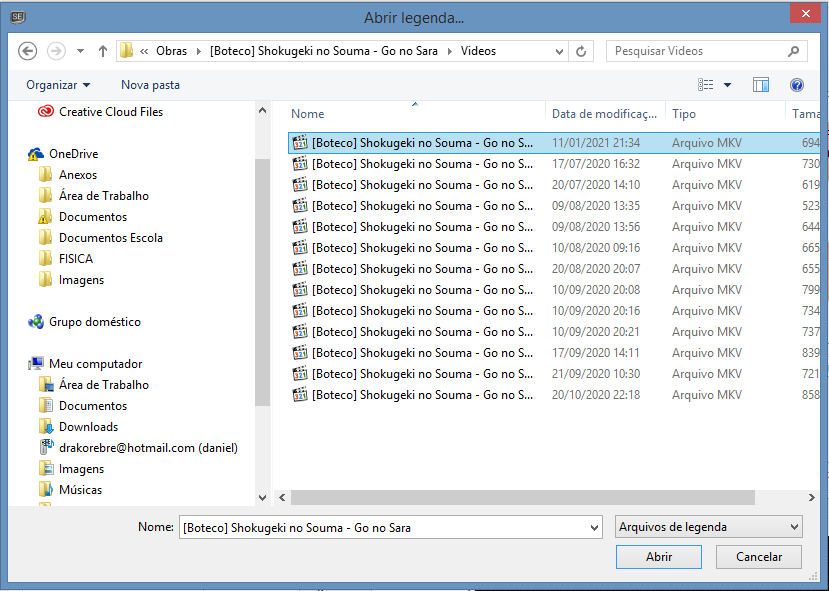
\includegraphics[width=0.85\textwidth]{Fig5.png}
 \caption{Selecionando um episódio dos \textit{animes} para exemplificar a extração das legendas.}
 \label{fig05}
 \source{Elaboração nossa.}
\end{figure}

\begin{figure}[htbp]
 \centering
 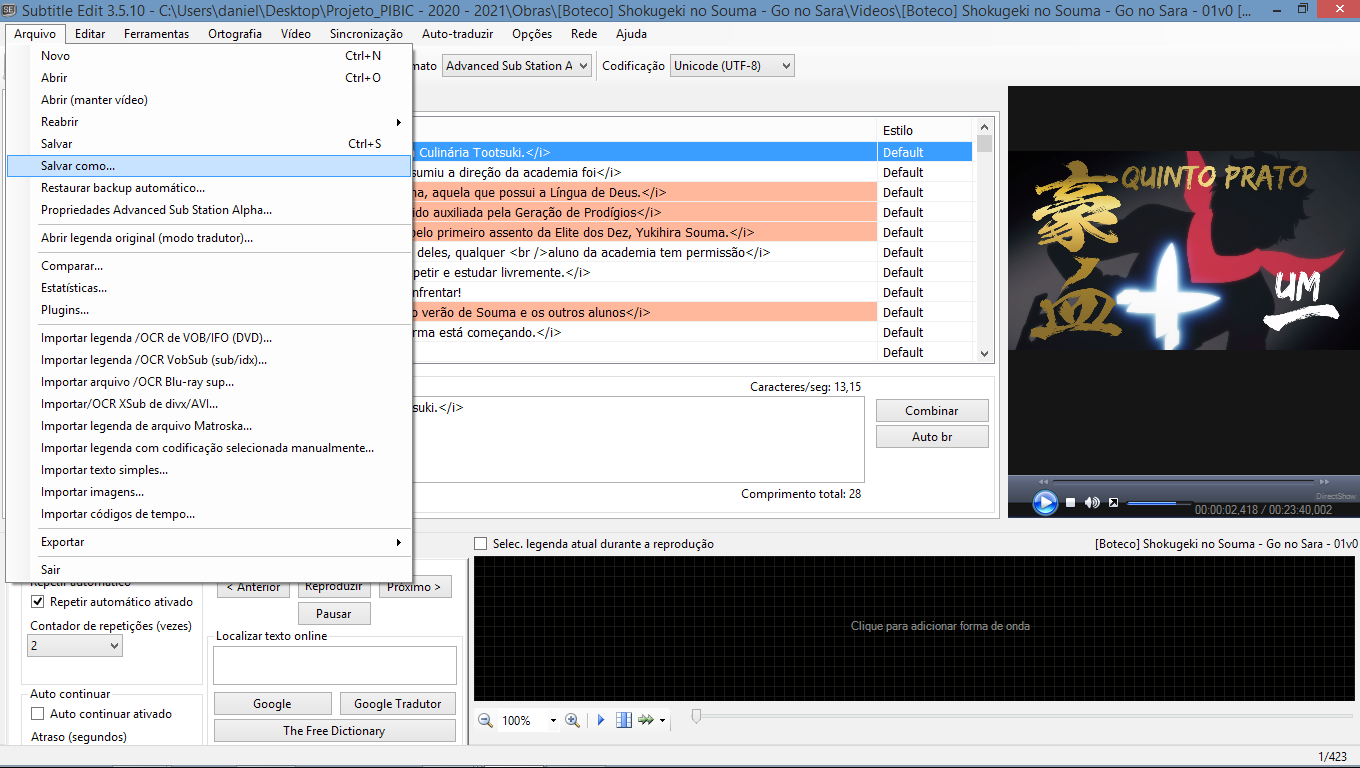
\includegraphics[width=0.85\textwidth]{Fig6.png}
 \caption{Realizando a extração da legenda de um episódio.}
 \label{fig06}
 \source{Elaboração nossa.}
\end{figure}

\begin{figure}[htbp]
 \centering
 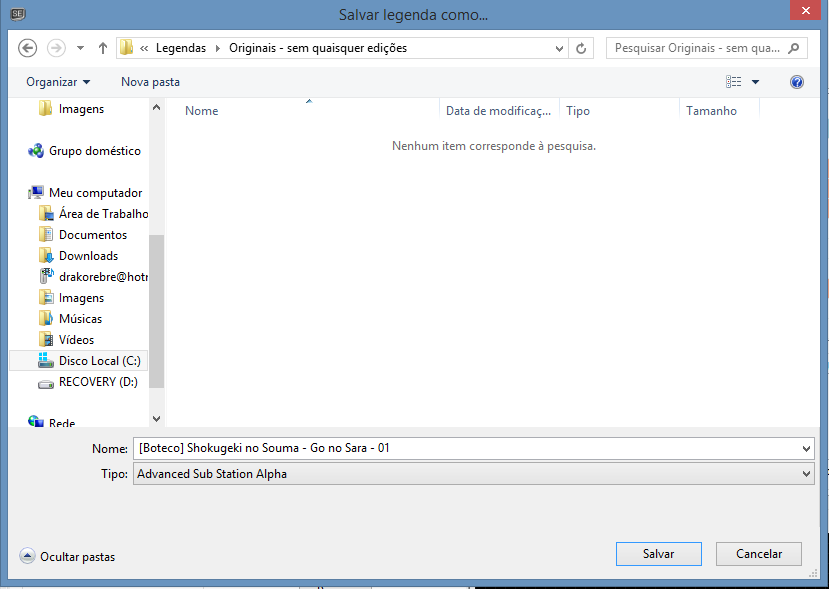
\includegraphics[width=0.85\textwidth]{Fig7.png}
 \caption{Salvando a legenda extraída em uma pasta específica dos arquivos da pesquisa.}
 \label{fig07}
 \source{Elaboração nossa.}
\end{figure}

\begin{figure}[htbp]
 \centering
 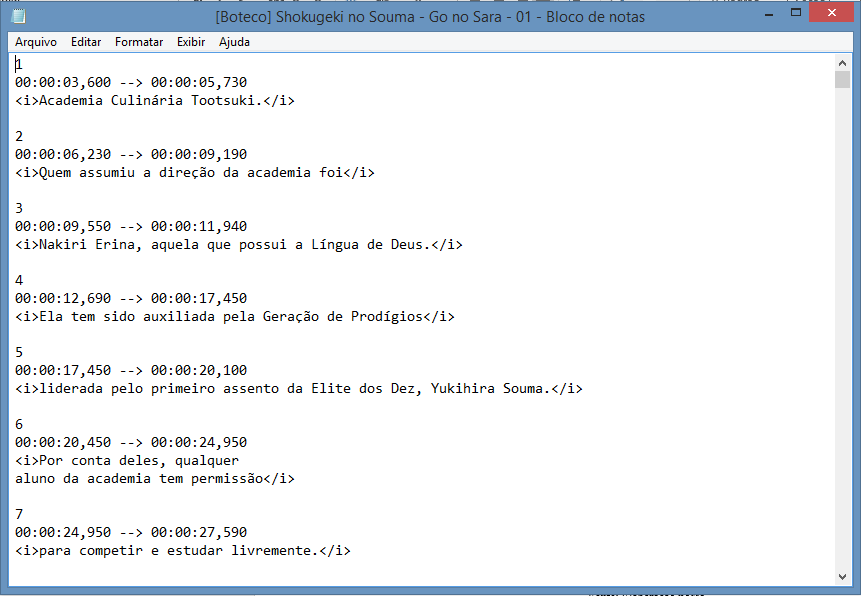
\includegraphics[width=0.85\textwidth]{Fig8.png}
 \caption{Trecho da legenda aberta no Bloco de Notas, após ser extraída no formato \textit{SubRip}, para exemplificar o processo de extração.}
 \label{fig08}
 \source{Elaboração nossa.}
\end{figure}

\subsection{Etapa de elaboração de códigos para identificar as obras}\label{sec-organizacao-latex}
Nesta etapa, com o material de estudo em mãos, seguimos com a nomeação dos arquivos de legendas (\Cref{fig09}). Para facilitar a identificação das obras, estabelecemos o padrão apresentado na \Cref{tbl3}.

\begin{table}[h!]
\caption{Critérios utilizados para nomear os episódios de \textit{anime} nos arquivos das pesquisas.}
\label{tbl3}
\centering
\begin{tabularx}{\linewidth}{XXXX}
\toprule
\textbf{Grupo} & \textbf{Nome da série} & \textbf{Temporada} & \textbf{Episódio} \\ 
\midrule
(Dois a três caracteres) & (Dois a três caracteres) & (Três caracteres) & (Três caracteres)
\\ 
{[}MM{]} & YU & T01 & E01
\\
{[}TDM{]} & KnT & T01 & E13
\\
\bottomrule
\end{tabularx}
\source{Elaboração nossa.}
\end{table}

[MM]YUT01E01 → Este código se refere ao grupo \textit{fansubber} MM (Moshi Moshi), que produziu legendas do \textit{anime} YU (\textit{Yesterday wo Utatte}), para a temporada 01 do episódio 01 desta série.

[TDM]KnTT01E13 → Este código se refere ao grupo \textit{fansubber} TDM, que produziu legendas do \textit{anime} KnT (\textit{Kami no Tou}), para a temporada 01 do episódio 13 desta série. 

\begin{figure}[htbp]
 \centering
 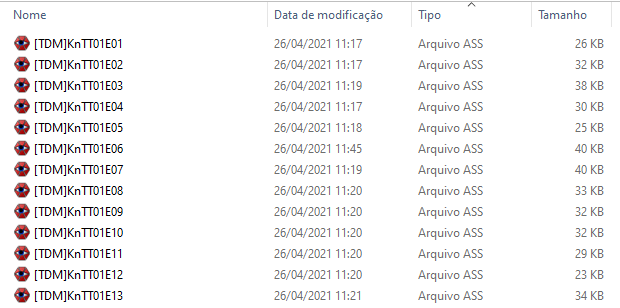
\includegraphics[width=0.85\textwidth]{Fig9.png}
 \caption{Lista dos episódios do \textit{anime}: ‘\textit{Kami no Tou}’, já nomeado.}
 \label{fig09}
 \source{Elaboração nossa.}
\end{figure}

Concluída a identificação dos episódios conforme os critérios definidos, avançamos para a próxima etapa das pesquisas, apresentada na \Cref{sec-titulo}. Nesta parte, estruturamos os arquivos de legendas antes de inclui-los no \textit{WordSmith Tools©}, v. 7.

\subsection{Preparação dos arquivos de legendas para inseri-las no WordList}\label{sec-titulo}
Efetuada a nomeação dos arquivos, avaliamos e tratamos os arquivos de legendas com um olhar especial às peculiaridades de cada grupo e cada obra de \textit{anime}, antes de ampliarmos o \textit{corpus} em si. Decidimos, por exemplo, utilizar o programa \textit{Aegisub}\footnote{Repositório GitHub: \url{https://github.com/Aegisub/Aegisub/releases}. Acesso em: 08 jul. 2021.} para colocar em angulares (< >) as legendas com palavras escritas em caracteres estrangeiros, ou legendas com frases em outros idiomas, algo que geralmente aparece durante a abertura e o encerramento de um \textit{anime}. Dessa forma, eles serão reconhecidos pelo \textit{WordList}, ferramenta disponibilizada pelo \textit{WordSmith Tools©}, e todos os caracteres que estão entre os angulares não servirão para contagem de palavras do \textit{corpus}. O que fundamentou esta decisão foi principalmente a língua utilizada nos textos a serem imputados no \textit{CorLeAni}: língua portuguesa. Em ambos os casos, de palavras escritas em caracteres estrangeiros e de legendas em outros idiomas que não o português brasileiro, são exemplificados a seguir, nas \Cref{fig10} e \Cref{fig11}, respectivamente.

\begin{figure}[htbp]
 \centering
 
\includegraphics[width=0.85\textwidth]{Fig10.png}
 \caption{Cena do \textit{anime Kimetsu no Yaiba} com palavras escritas em caracteres estrangeiros ao português brasileiro.}
 \label{fig10}
 \source{Elaboração nossa.}
\end{figure}

\begin{figure}[htbp]
 \centering
 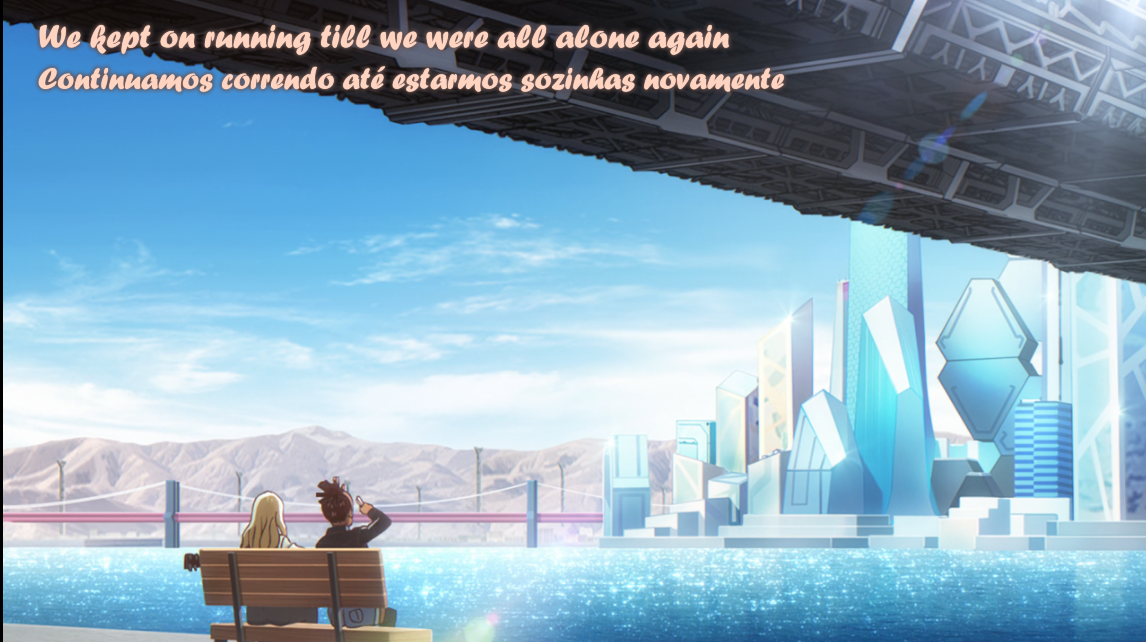
\includegraphics[width=0.85\textwidth]{Fig11.png}
 \caption{Cena do \textit{anime Carole \& Tuesday} com legendas em português e inglês.}
 \label{fig11}
 \source{Elaboração nossa.}
\end{figure}

Especificamente no PIBIC-EM 2020-2021, essa decisão só foi aplicada ao grupo \textit{fansubber} “\textit{Elite}”, pois foi o único grupo que realizou a transcrição e tradução da abertura e do encerramento do \textit{anime} intitulado: “\textit{Appare-Ranman!}” (\Cref{fig12}).

\begin{figure}[htbp]
 \centering
 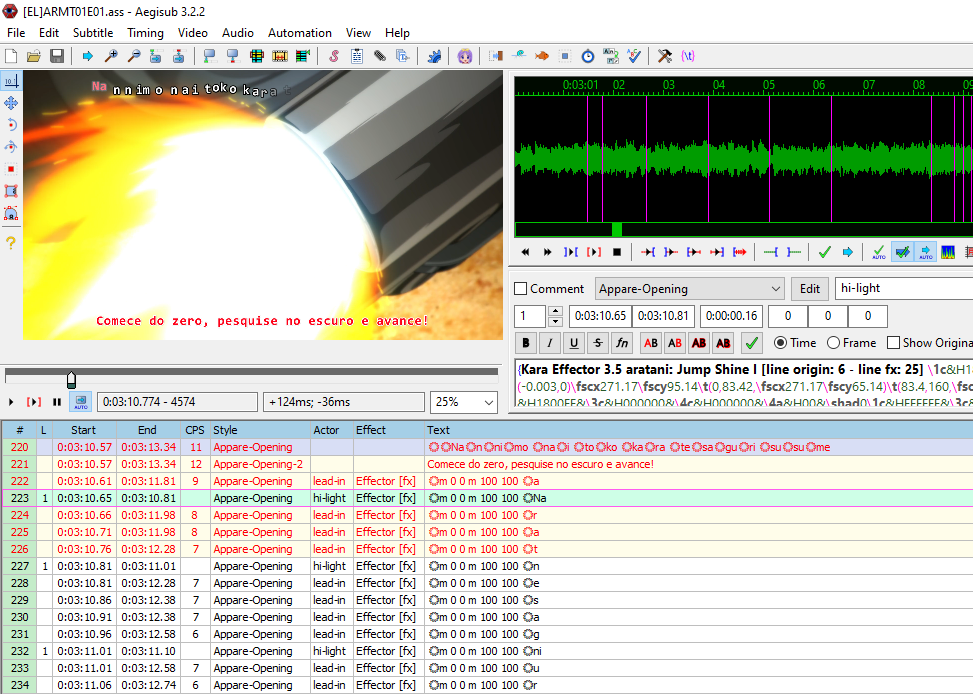
\includegraphics[width=0.85\textwidth]{Fig12.png}
 \caption{Transcrição da abertura do \textit{anime} “\textit{Appare-Ranman}” em karaokê.}
 \label{fig12}
 \source{Elaboração nossa.}
\end{figure}

Estabelecemos, também, um outro critério para definir a ordem em que as linhas de legendas aparecem nos arquivos. Percebemos que o padrão do \textit{software} é organizar as linhas de legendas conforme elas são criadas, como é exemplificado na \Cref{tbl5}. Contudo, preferimos organizá-las pela ordem alfabética do nome dos estilos estabelecidos pelos \textit{fansubbers}, conforme a \Cref{tbl4}.

\begin{table}[htbp]
\caption{Representação de legendas na ordem alfabética dos estilos que foram preestabelecidos no arquivo de legenda.}
\label{tbl4}
\centering
\begin{tabularx}{\linewidth}{XXXXX}
\toprule
\textbf{Linha} & \textbf{Tempo inicial} & \textbf{Tempo final} & \textbf{Estilo} & \textbf{Texto} \\ 
\midrule
1 & 00:38 & 00:40 & Legenda-Inferior & Olá.
\\ 
2 & 00:46 & 00:51 & Legenda-Inferior & Que isso, o prazer é todo meu.
\\
3 & 00:40 & 00:43 & Legenda-Superior & Olá! Prazer em conhecê-lo.
\\
\bottomrule
\end{tabularx}
\source{Elaboração nossa.}
\end{table}

\begin{table}[h!]
\caption{Representação de legendas na ordem em que foram inseridas no arquivo de legenda.}
\label{tbl5}
\centering
\begin{tabularx}{\linewidth}{XXXXX}
\toprule
\textbf{Linha} & \textbf{Tempo inicial} & \textbf{Tempo final} & \textbf{Estilo} & \textbf{Texto} \\ 
\midrule
1 & 00:38 & 00:40 & Legenda-Inferior & Olá.
\\ 
2 & 00:40 & 00:43 & Legenda-Superior & Olá! Prazer em conhecê-lo.
\\
3 & 00:46 & 00:51 & Legenda-Inferior & Que isso, o prazer é todo meu.
\\
\bottomrule
\end{tabularx}
\source{Elaboração nossa.}
\end{table}

Dessa forma, as linhas que têm uma característica em comum ficam organizadas próximas umas das outras, a depender do estilo que foi determinado pelo \textit{fansubber}. A decisão foi tomada para facilitar e ajudar na análise e no processo de inserção de angulares nas legendas. É importante ressaltar que, quando olhamos no arquivo de legenda à primeira vista, as legendas podem parecer estar desorganizadas ou dessincronizadas, conforme observamos na \Cref{tbl4}. No entanto, se vincularmos esses arquivos de legendas a um arquivo de vídeo qualquer, ou ao próprio episódio do \textit{anime}, perceberemos que elas ainda serão apresentadas para o espectador da mesma forma que o arquivo de legenda dos \textit{fansubbers} originalmente apresentaria. O tempo, responsável por definir em que momentos as legendas devem aparecer ou sair da tela, não foi alterado, mas sim o critério que organiza as linhas de legenda no arquivo (nesse caso, o estilo das legendas).

Na \Cref{fig13}, apresentamos o programa de legendagem \textit{Aegisub} (versão 3.2.2), que, entre tantas funções, organiza as legendas pela ordem alfabética dos estilos. Nas \Cref{fig14} e \Cref{fig15}, mostramos a frase “Ei, você, espere aí!” antes (\Cref{fig14}, em um arquivo de legenda, sem alteração no conteúdo) e depois (\Cref{fig15}) de mudar o critério que define a ordem das legendas no arquivo. 

\begin{figure}[htbp]
 \centering
 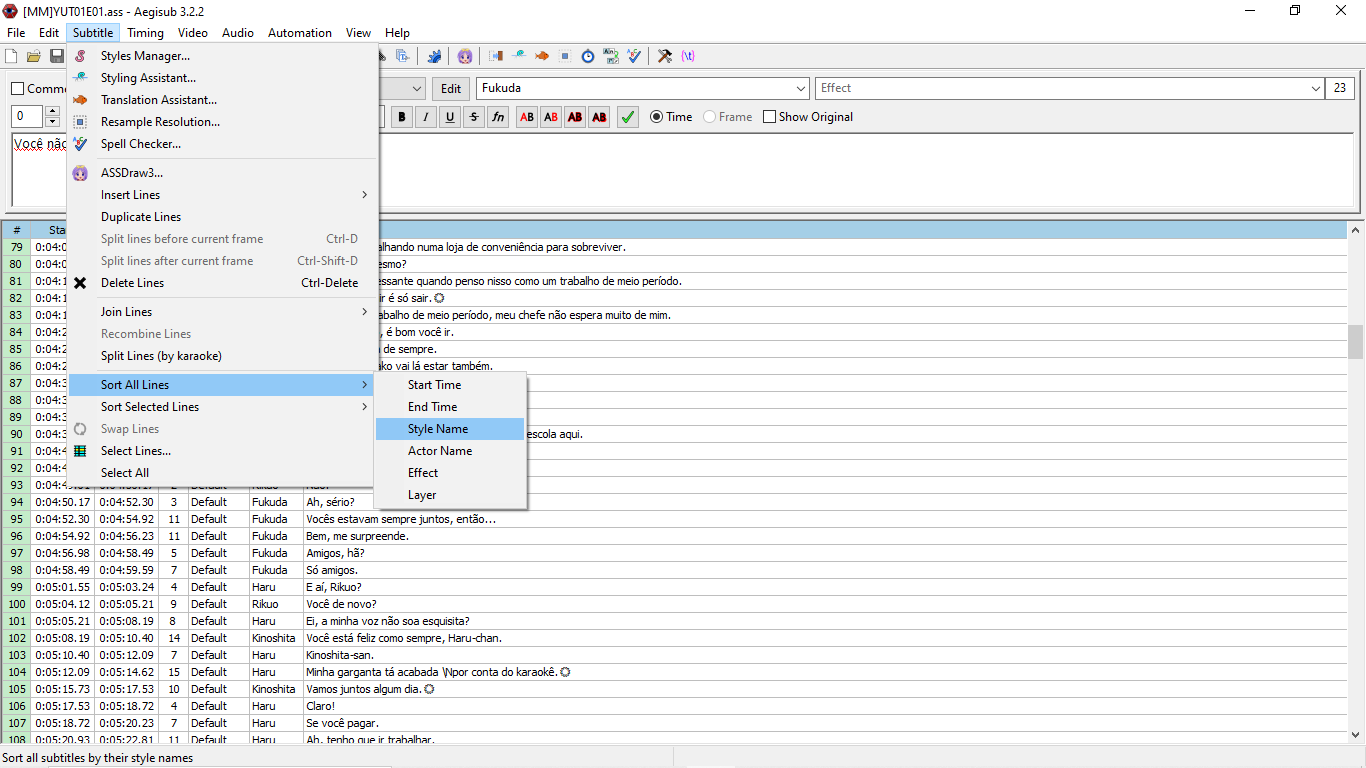
\includegraphics[width=0.85\textwidth]{Fig13.png}
 \caption{Organizando as legendas pelo nome dos estilos pré-definidos pelos \textit{fansubbers}.}
 \label{fig13}
 \source{Elaboração nossa.}
\end{figure}

\begin{figure}[htbp]
 \centering
 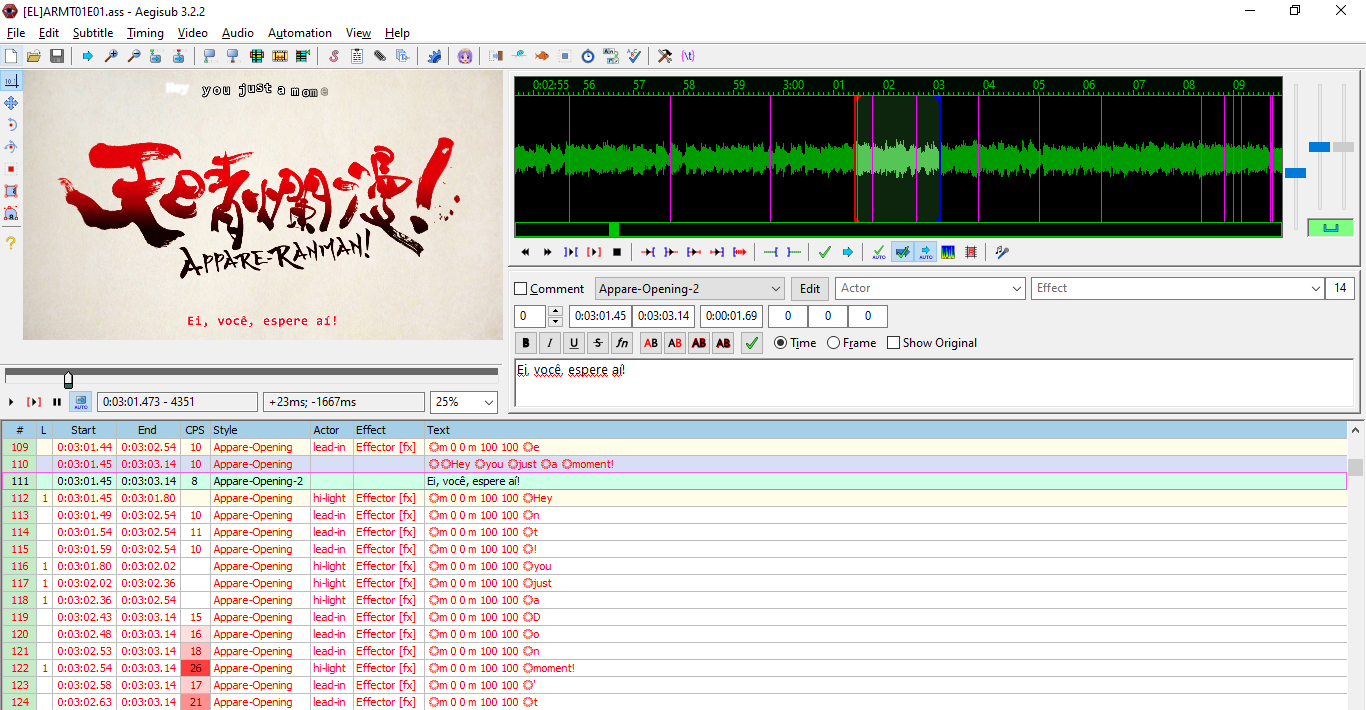
\includegraphics[width=0.85\textwidth]{Fig14.png}
 \caption{Arquivo de legenda após a extração, com legendas organizadas no formato padrão. A linha 110 está comentada e as outras apresentam karaokê e códigos de formatação.}
 \label{fig14}
 \source{Elaboração nossa.}
\end{figure}

\begin{figure}[htbp]
 \centering
 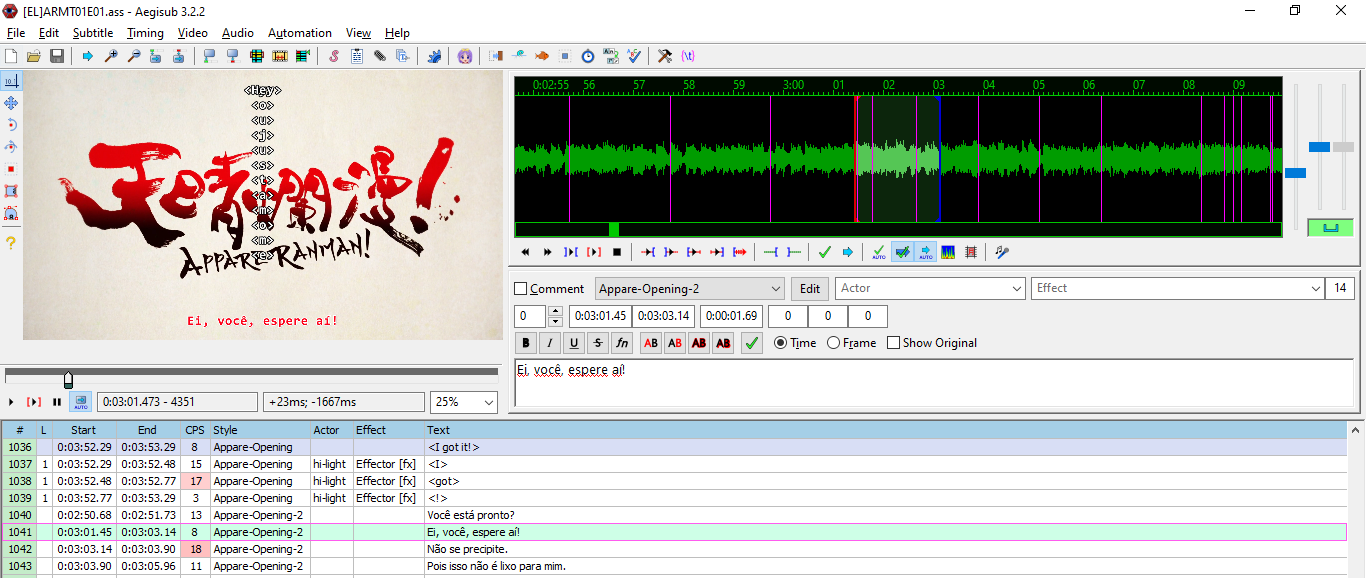
\includegraphics[width=0.85\textwidth]{Fig15.png}
 \caption{Legendas organizadas pela ordem alfabética dos estilos, com palavras estrangeiras e karaokê (linha 1036 a 1039) em angular.}
 \label{fig15}
 \source{Elaboração nossa.}
\end{figure}

Observamos, a partir da análise, que mesmo quando o número da linha da frase tenha sido alterado no arquivo de legenda (\Cref{fig15}), as legendas continuam sendo exibidas para o telespectador no tempo definido pelos \textit{fansubbers} (\Cref{fig14}). Outra coisa observada, na \Cref{fig15}, são as legendas que aparecem entre os angulares (< >), códigos não assimilados pelo \textit{Aegisub}. Analisando essas imagens, é possível inferir, ainda, que optamos por retirar os códigos de formatação dos arquivos de legenda, assunto abordado na \Cref{sec-autores}.

Uma outra decisão que tomamos se trata dos comentários feitos pelos \textit{fansubbers}, característica bastante presente nesse tipo de legenda \cite{diaz-cintas_fansubs:_2006}. Neste caso, decidimos recorrer uma vez mais aos angulares para que essas ocorrências não sejam contabilizadas no \textit{corpus}. Por comentários, nós entendemos legendas ou frases que não são exibidas para o telespectador, mas que servem como forma de comunicação entre os \textit{fansubbers}. Em alguns casos, há a presença de \textit{links} de \textit{sites} (\Cref{fig16}) ou palavras escritas em caracteres estrangeiros, mas que são, em sua maioria, diálogos ou observações feitas entre ou para os próprios \textit{fansubbers}. 

\begin{figure}[htbp]
 \centering
 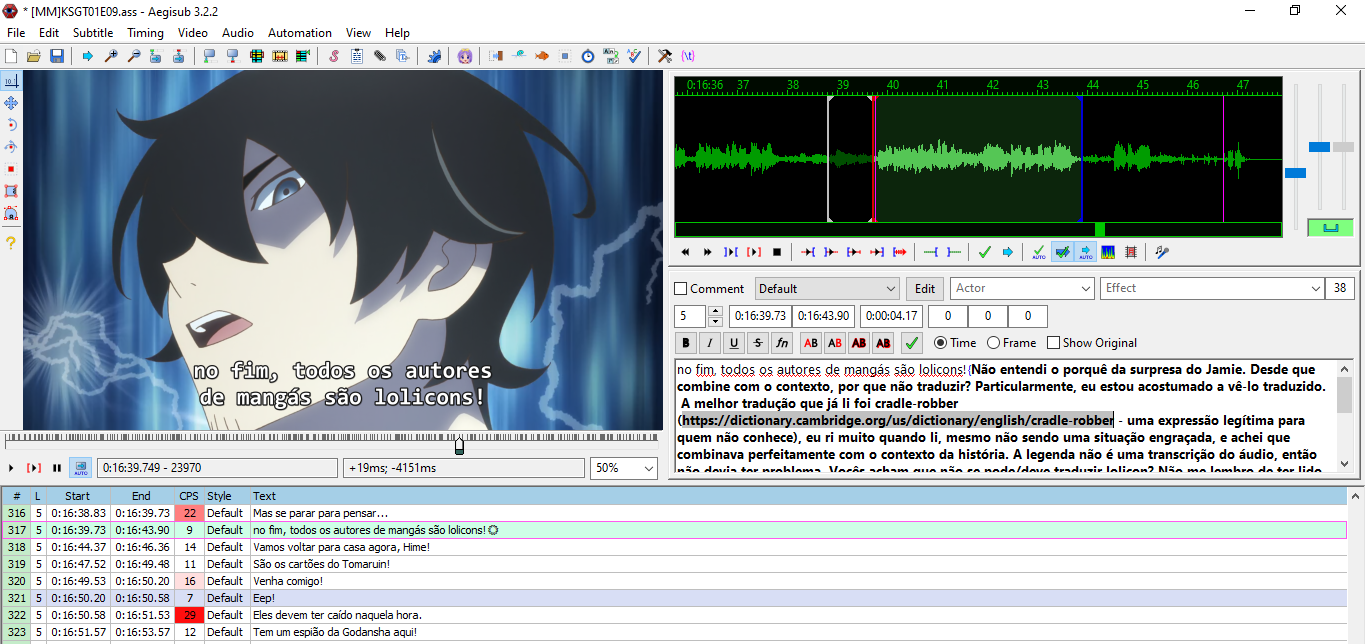
\includegraphics[width=0.85\textwidth]{Fig16.png}
 \caption{Exemplo de comentários (linhas 317 e 321) que não são exibidos para o espectador, ainda sem angular, que contém o \textit{link} de um \textit{site}.}
 \label{fig16}
 \source{Elaboração nossa.}
\end{figure}

\subsubsection{Exportação personalizada e uso da ferramenta conversão em lote}\label{sec-autores}
Como foi brevemente abordado, optamos por excluir os códigos de formatação presentes nos arquivos de legendas. No projeto PIBIC-EM 2019-2020, também tomamos essa decisão e avaliamos que, na pesquisa PIBIC-EM 2020-2021, essa escolha continuaria sendo válida, embora tenhamos encontrado uma quantidade consideravelmente menor de códigos de formatação. Contudo, ainda nos deparamos com outros códigos encontrados na primeira pesquisa, à exceção daqueles que eram, na verdade, palavras. Preferimos, portanto, utilizar um formato de texto personalizado, pois facilitaria a padronização dos cabeçalhos e tornaria mais prático o processo de colocar entre angulares o número das linhas e os tempos de início e fim de uma linha de legenda.

A ferramenta ‘conversão em lote’, do programa \textit{Subtitle Edit}, também foi utilizada para conseguirmos retirar alguns códigos que o \textit{Aegisub} destaca com um símbolo “\inlinegraphics{simbolo.png}”, como é exemplificado nas linhas 342 a 344 da \Cref{fig17}. Quanto aos códigos como os que são apresentados nas linhas 112 a 119 (onde aparece “m 0 0 m 100 100”), na \Cref{fig14}, tivemos que optar por realizar uma remoção manual. Todo esse processo de configurar um formato de texto personalizado, a partir da ferramenta \textit{conversão em lote}, no \textit{Subtitle Edit}, e o uso da própria ferramenta para remover alguns códigos de formatação específicos até a obtenção do arquivo final em bloco de notas, estão exemplificados nas \Cref{fig17}, \Cref{fig18}, \Cref{fig19}, \Cref{fig20}, \Cref{fig21}, \Cref{fig22}, \Cref{fig23}, \Cref{fig24}, \Cref{fig25}, \Cref{fig26} e \Cref{fig27}.

\begin{figure}[htbp]
 \centering
 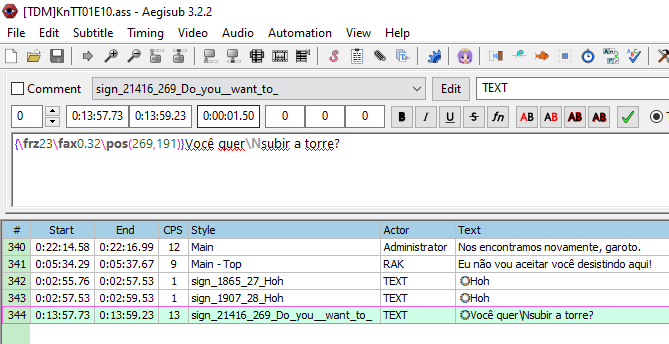
\includegraphics[width=0.85\textwidth]{Fig17.png}
 \caption{Código de efeitos nas linhas de legendas.}
 \label{fig17}
 \source{Elaboração nossa.}
\end{figure}

\begin{figure}[htbp]
 \centering
 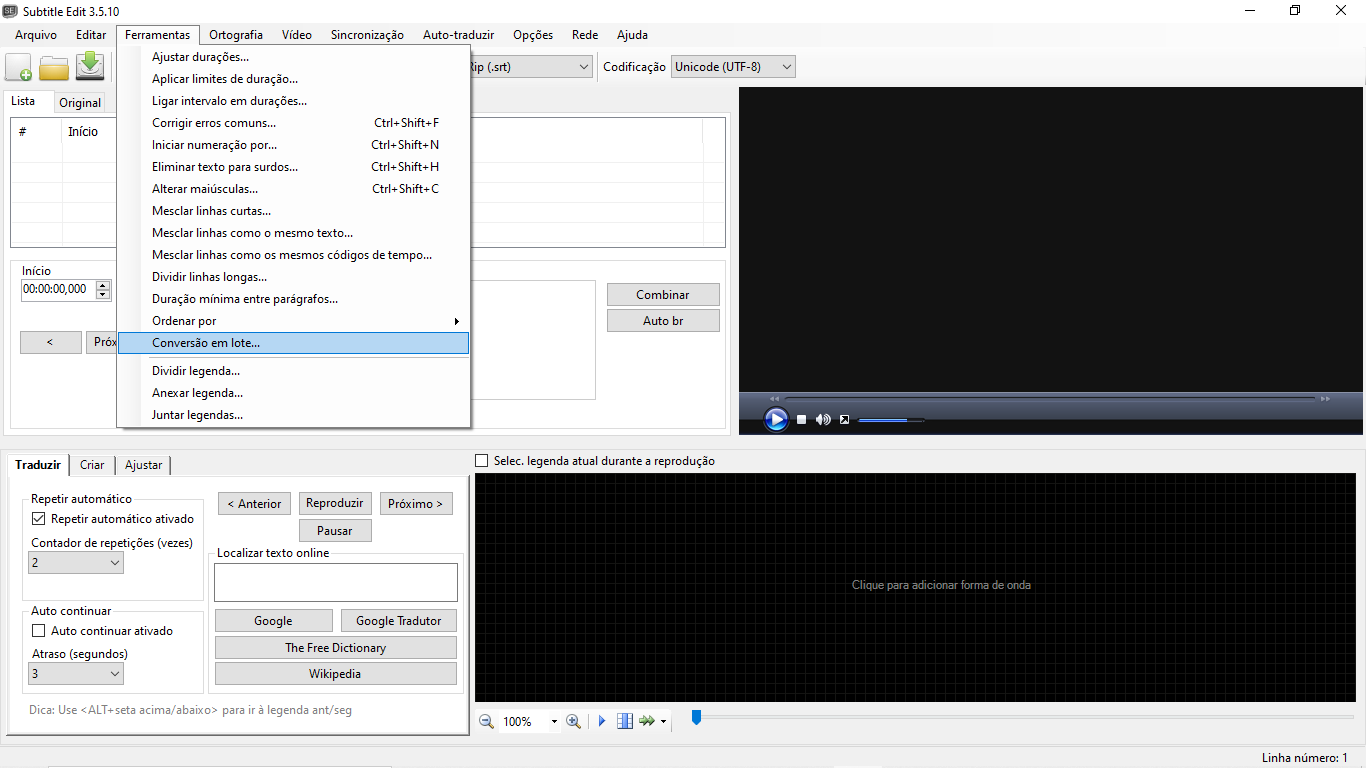
\includegraphics[width=0.85\textwidth]{Fig18.png}
 \caption{Abrindo a ferramenta “Conversão em lote” na interface do \textit{Subtitle Edit}.}
 \label{fig18}
 \source{Elaboração nossa.}
\end{figure}

\begin{figure}[htbp]
 \centering
 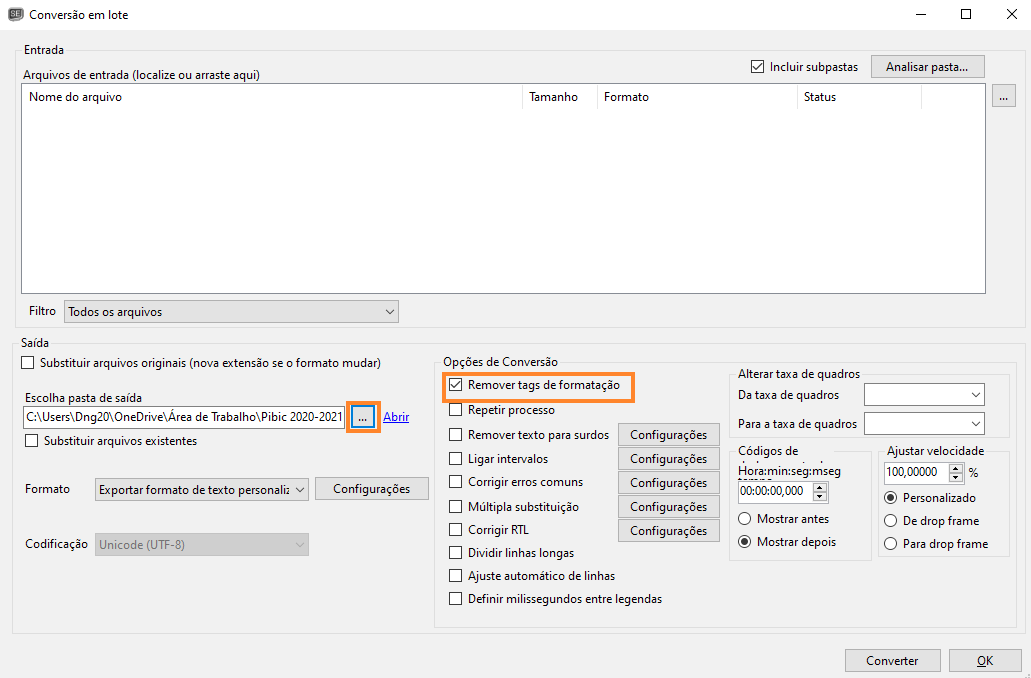
\includegraphics[width=0.85\textwidth]{Fig19.png}
 \caption{Selecionando a opção “Remover \textit{tags} de formatação” 
e definindo a pasta onde os arquivos convertidos serão salvos.}
 \label{fig19}
 \source{Elaboração nossa.}
\end{figure}

\begin{figure}[htbp]
 \centering
 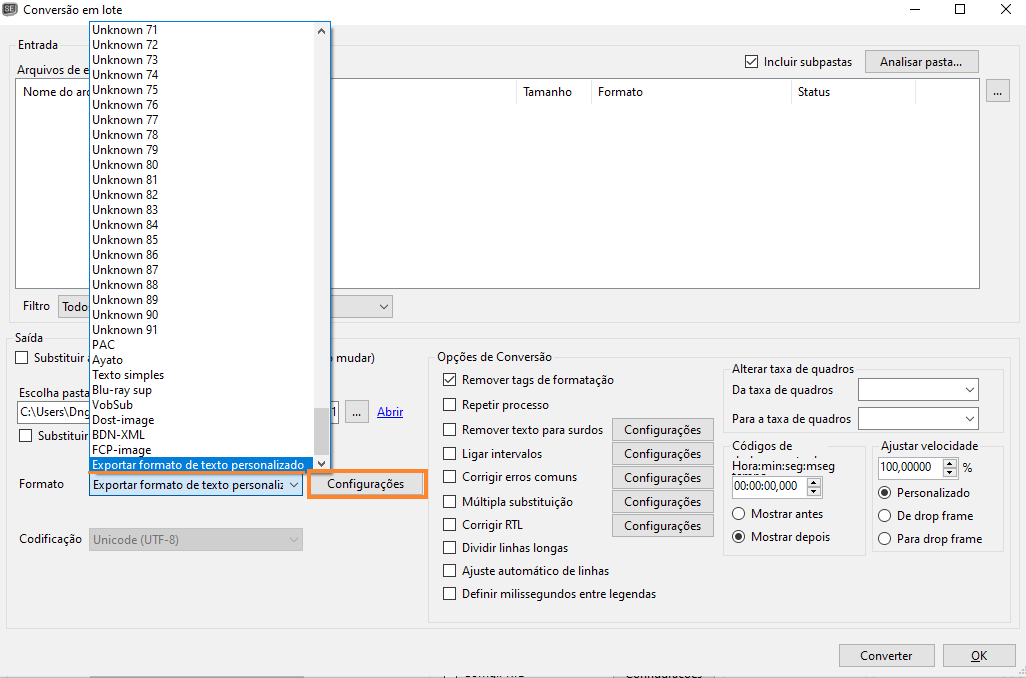
\includegraphics[width=0.85\textwidth]{Fig20.png}
 \caption{Selecionando a opção para exportar um formato de texto personalizado  e abrindo as configurações para exportação de formato de texto personalizado.}
 \label{fig20}
 \source{Elaboração nossa.}
\end{figure}

\begin{figure}[htbp]
 \centering
 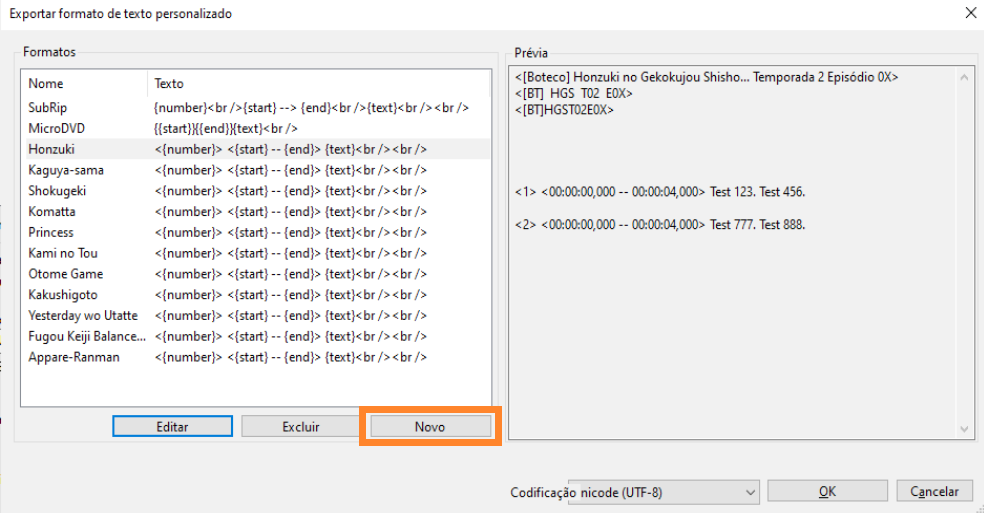
\includegraphics[width=0.85\textwidth]{Fig21.png}
 \caption{Criando um novo formato de texto personalizado.}
 \label{fig21}
 \source{Elaboração nossa.}
\end{figure}

\begin{figure}[htbp]
 \centering
 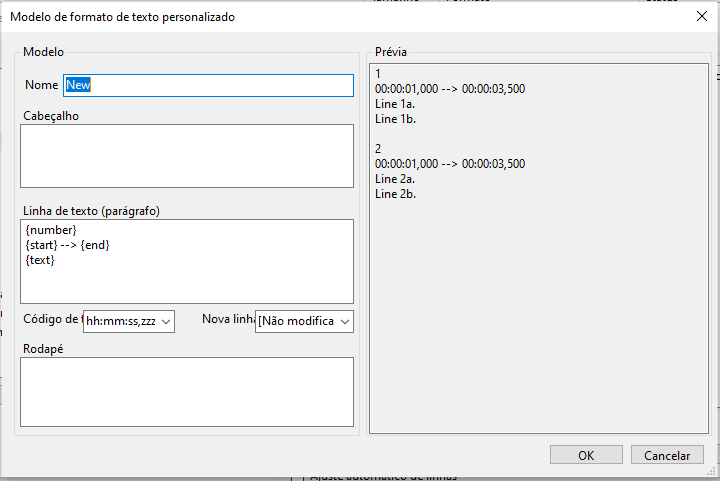
\includegraphics[width=0.85\textwidth]{Fig22.png}
 \caption{Interface para a configuração de um formato de texto personalizado.}
 \label{fig22}
 \source{Elaboração nossa.}
\end{figure}

\begin{figure}[htbp]
 \centering
 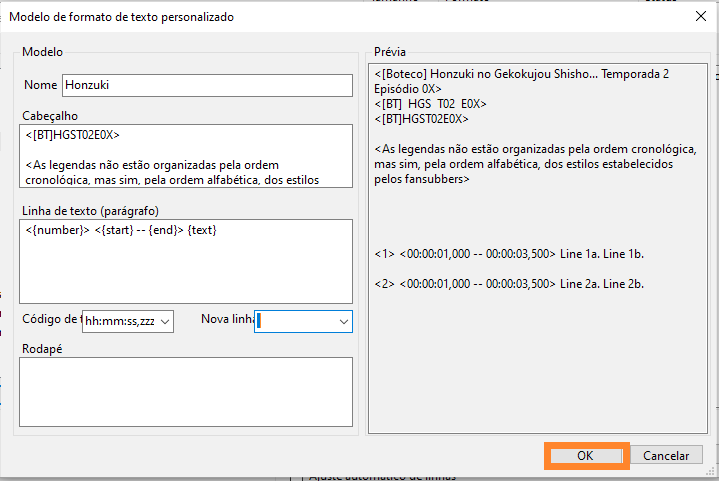
\includegraphics[width=0.85\textwidth]{Fig23.png}
 \caption{Novo formato de texto após ser configurado.}
 \label{fig23}
 \source{Elaboração nossa.}
\end{figure}

\begin{figure}[htbp]
 \centering
 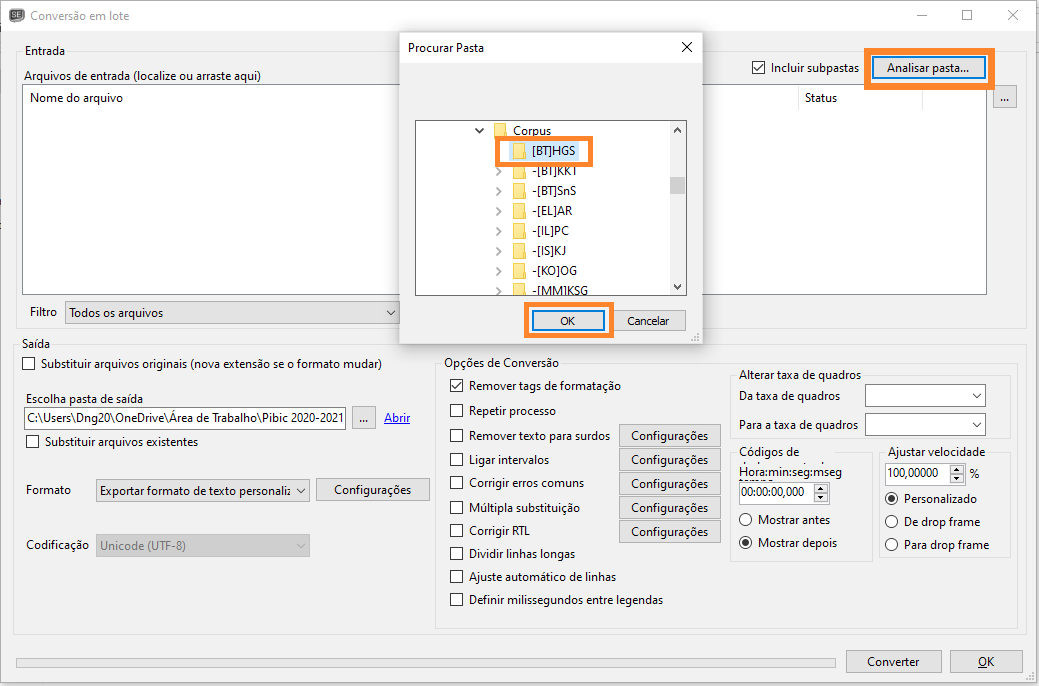
\includegraphics[width=0.85\textwidth]{Fig24.png}
 \caption{Selecionando pasta com as legendas a serem convertidas.}
 \label{fig24}
 \source{Elaboração nossa.}
\end{figure}

\begin{figure}[htbp]
 \centering
 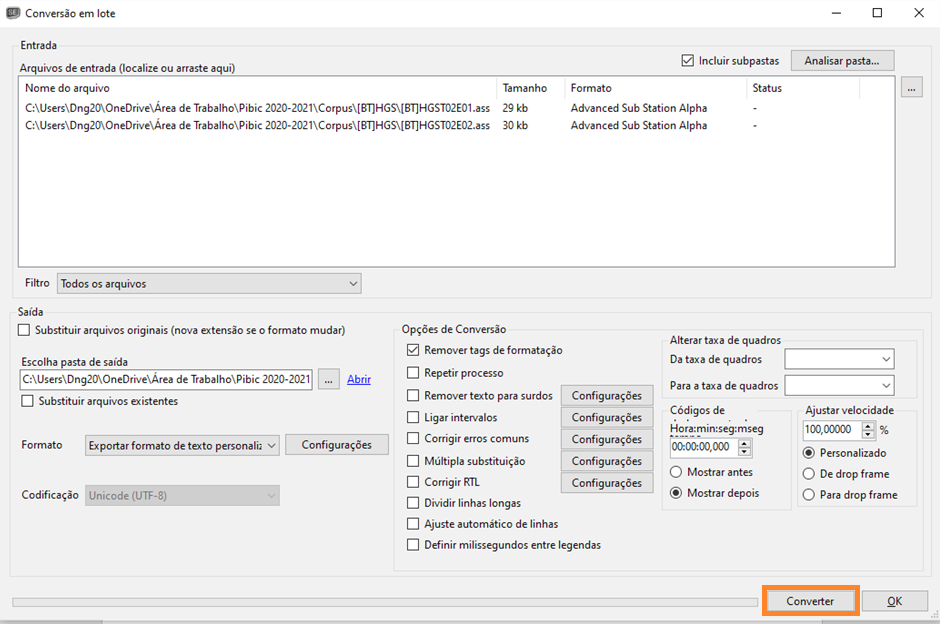
\includegraphics[width=0.85\textwidth]{Fig25.png}
 \caption{Legendas prontas para serem convertidas.}
 \label{fig25}
 \source{Elaboração nossa.}
\end{figure}

\begin{figure}[htbp]
 \centering
 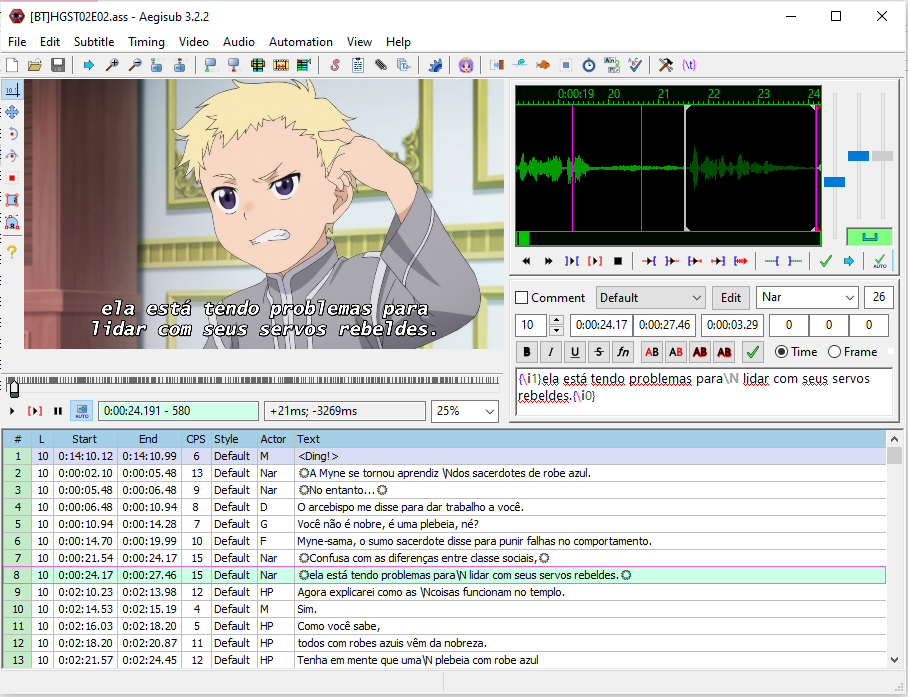
\includegraphics[width=0.85\textwidth]{Fig26.png}
 \caption{Arquivo de legenda antes da exportação.}
 \label{fig26}
 \source{Elaboração nossa.}
\end{figure}

\begin{figure}[htbp]
 \centering
 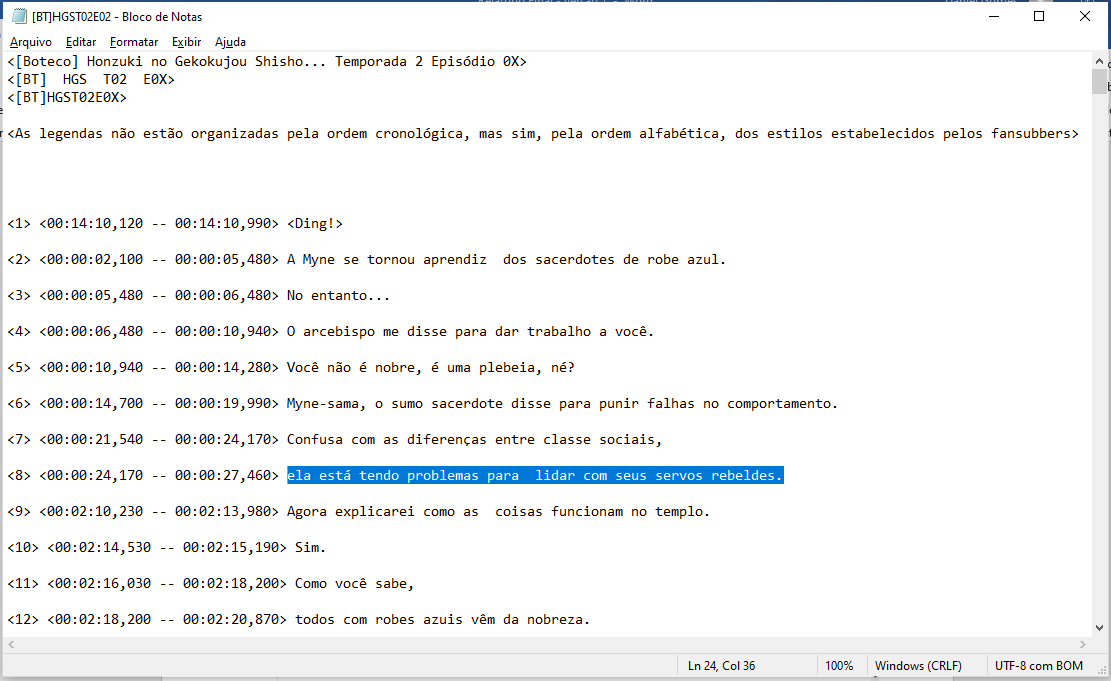
\includegraphics[width=0.85\textwidth]{Fig27.png}
 \caption{Arquivo de legenda após a exportação.}
 \label{fig27}
 \source{Elaboração nossa.}
\end{figure}

Olhando para a linha 8 na \Cref{fig26} (antes) e para essa mesma linha na \Cref{fig27} (depois), conseguimos perceber que as \textit{tags} de formatação foram removidas do arquivo de legenda. Destacamos que ambos os programas de legendagem supramencionados têm funções que não foram exploradas por estas pesquisas por fugirem aos interesses presentes, embora reconheçamos que algumas delas podem facilitar processos de padronização, como também de substituição de padrões. A ferramenta \textit{conversão em lote}, por exemplo, poderia ser empregada para aplicar uma substituição múltipla de determinadas palavras ou códigos, tomando diversos arquivos de uma só vez, a depender do contexto. Porém, preferimos nos limitar às funções apresentadas, pois já nos trouxeram resultados satisfatórios. 

\subsection{Cabeçalhos dos arquivos de legendas}\label{sec-idioma}
Utilizando o processo relatado no tópico anterior como vantagem, padronizamos a maioria dos cabeçalhos das legendas para cada obra, e, ao fim da conversão, os cabeçalhos já estavam em padrões pré-definidos. As \Cref{fig28} e \Cref{fig29} exemplificam esse processo no \textit{anime Fruits Basket}, traduzido pelo grupo \textit{Aenianos}.

\begin{figure}[htbp]
 \centering
 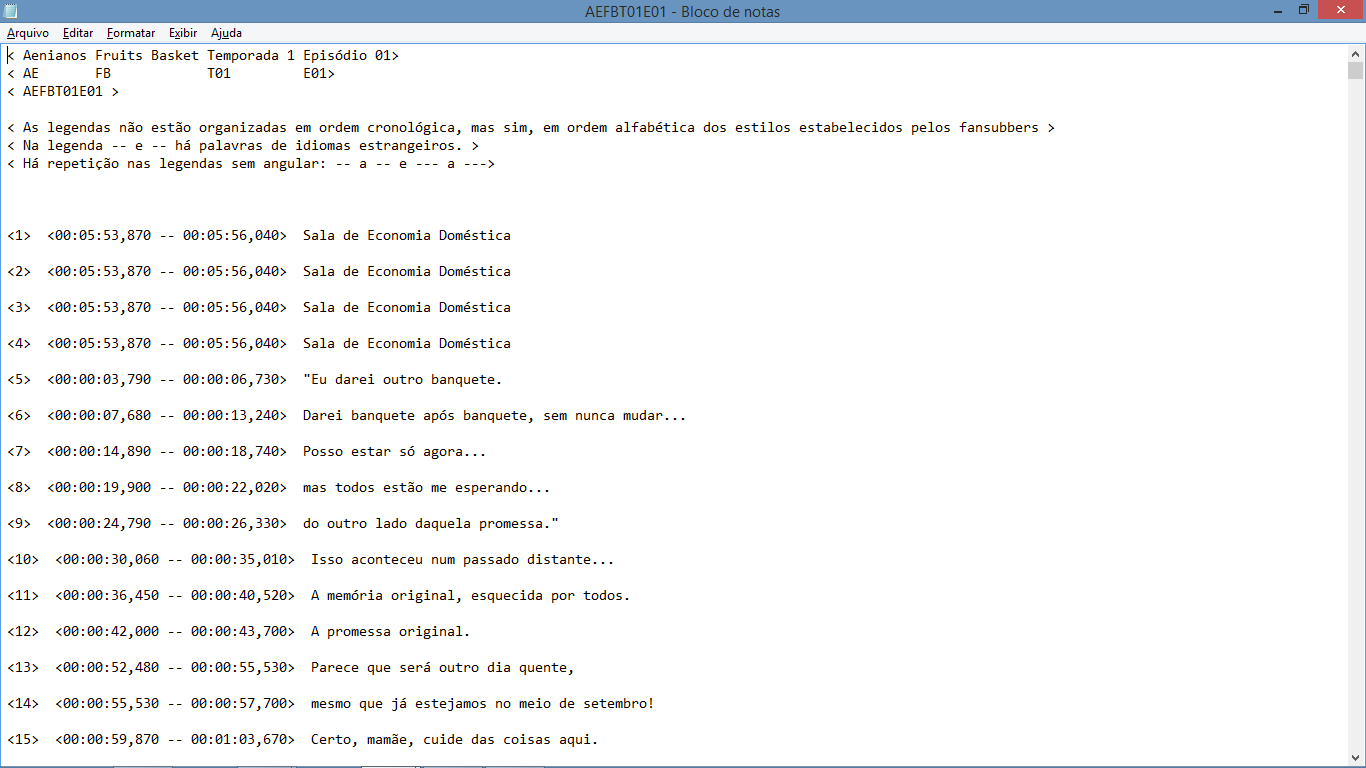
\includegraphics[width=0.85\textwidth]{Fig28.png}
 \caption{Cabeçalho pré-definido do exemplo do processo realizado na conversão em lote.}
 \label{fig28}
 \source{Elaboração nossa.}
\end{figure}

\begin{figure}[htbp]
 \centering
 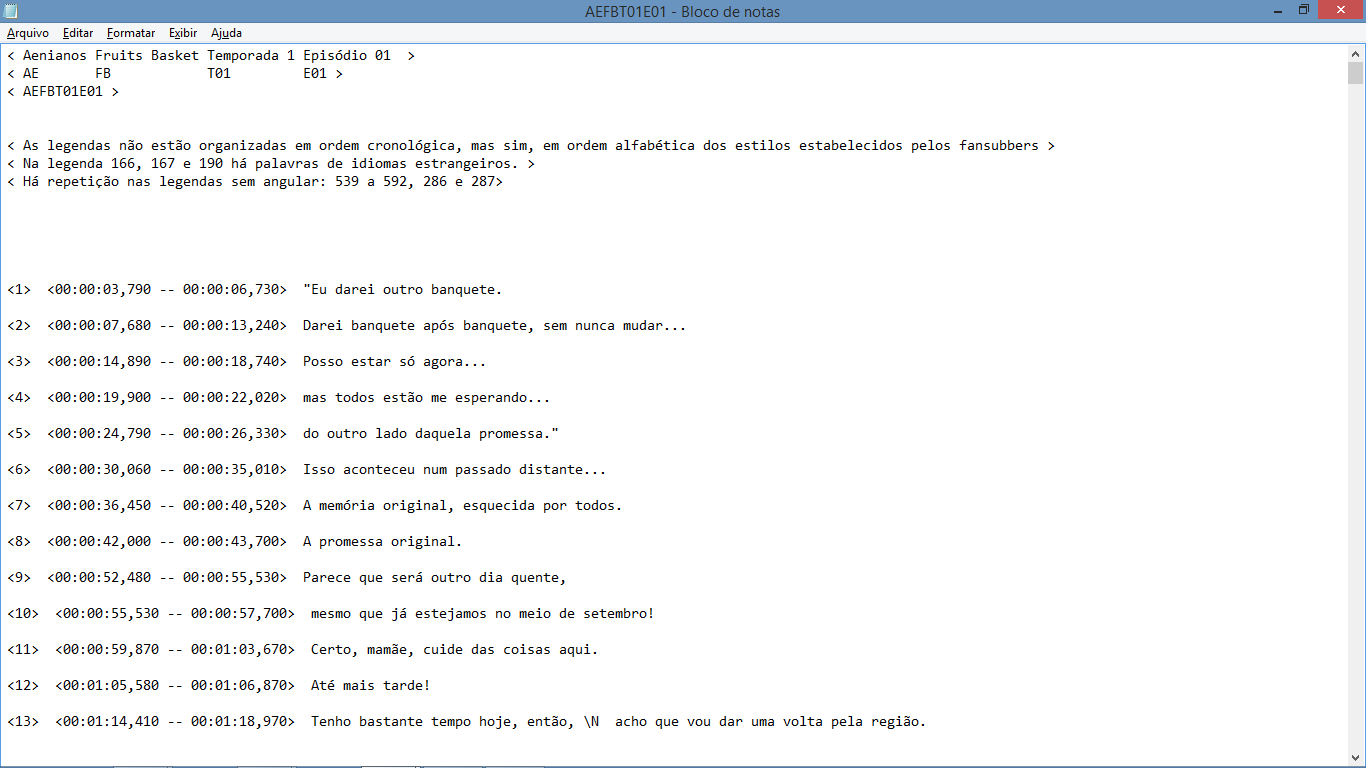
\includegraphics[width=0.85\textwidth]{Fig29.png}
 \caption{Cabeçalho do episódio 1 do \textit{anime} “\textit{Fruits Basket}”.}
 \label{fig29}
 \source{Elaboração nossa.}
\end{figure}

No geral, colocamos nas etiquetas informações que dizem respeito à duplicação de legendas, e indicamos as legendas onde há palavras estrangeiras ou que fazem referência a uma, como demonstrado na \Cref{fig30}. Além disso, compõem os cabeçalhos os seguintes dados: o nome do grupo de \textit{fansubbers}, o nome do \textit{anime}, a temporada e o episódio em extenso, dos quais surge o código do episódio, também presente nos cabeçalhos e que pode ser visto nas \Cref{fig28} e \Cref{fig29}.

\begin{figure}[htbp]
 \centering
 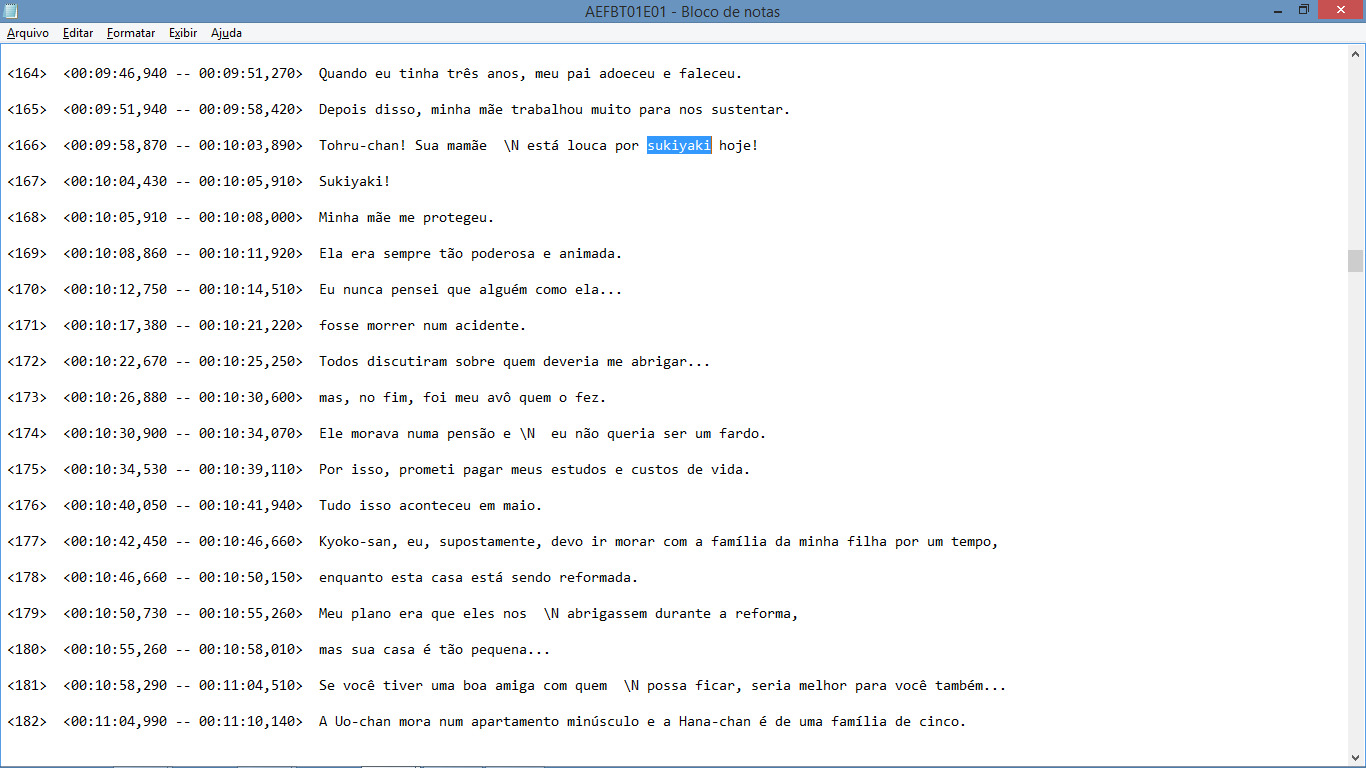
\includegraphics[width=0.85\textwidth]{Fig30.png}
 \caption{Palavra “\textit{sukiyaki}” indicada no cabeçalho do episódio 1 do \textit{anime} “\textit{Fruits Basket}” como uma palavra estrangeira.}
 \label{fig30}
 \source{Elaboração nossa.}
\end{figure}

Tendo percorrido todos os passos metodológicos relatados até então, os arquivos já se encontravam aptos a serem imputados na ferramenta \textit{WordList} do \textit{WordSmith Tools©} (versão 7). O procedimento seguinte consistiu em  criarmos a lista de palavras e obtermos os dados estatísticos do \textit{CorLeAni}.

\subsection{Consolidando o CorLeAni com auxílio do \textit{WordSmith Tools}}

Nesta etapa da pesquisa, foi feito o uso do WordSmith Tools para compilação do corpus, conforme exemplificado de forma resumida, nas \Cref{fig31}, \Cref{fig32} e \Cref{fig33}.

\begin{figure}[htbp]
 \centering
 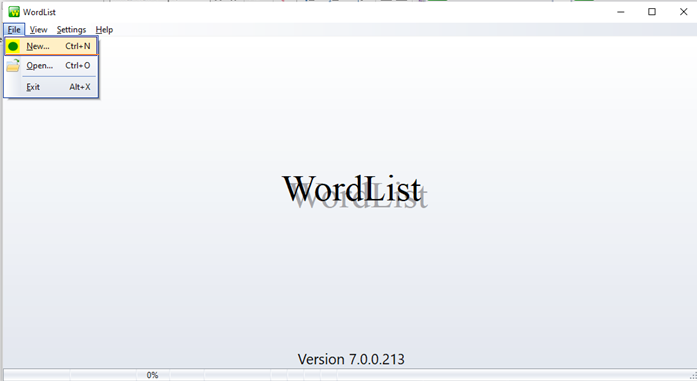
\includegraphics[width=0.85\textwidth]{Fig31.png}
 \caption{Interface do \textit{WordList}.}
 \label{fig31}
 \source{Elaboração nossa.}
\end{figure}

\begin{figure}[htbp]
 \centering
 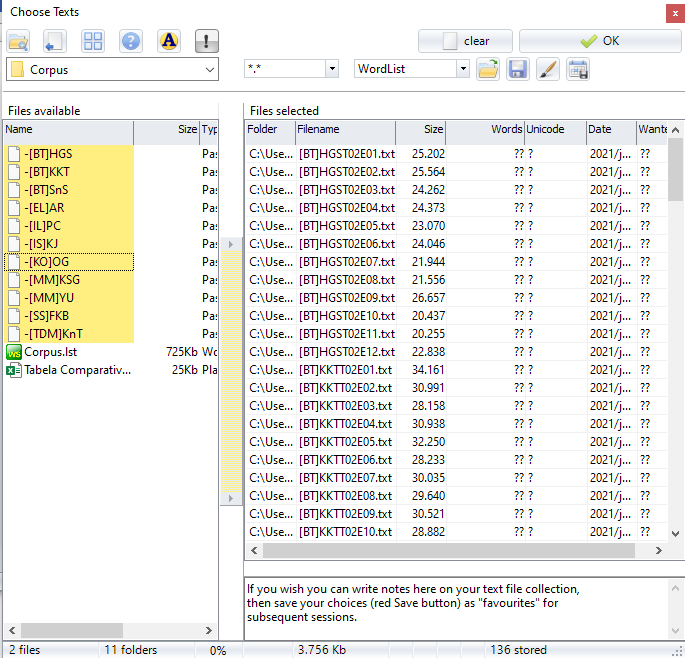
\includegraphics[width=0.85\textwidth]{Fig32.png}
 \caption{Indicando o diretório dos arquivos de legenda  para gerar uma lista de palavras (exemplo: textos do PIBIC 2020-2021).}
 \label{fig32}
 \source{Elaboração nossa.}
\end{figure}

\begin{figure}[htbp]
 \centering
 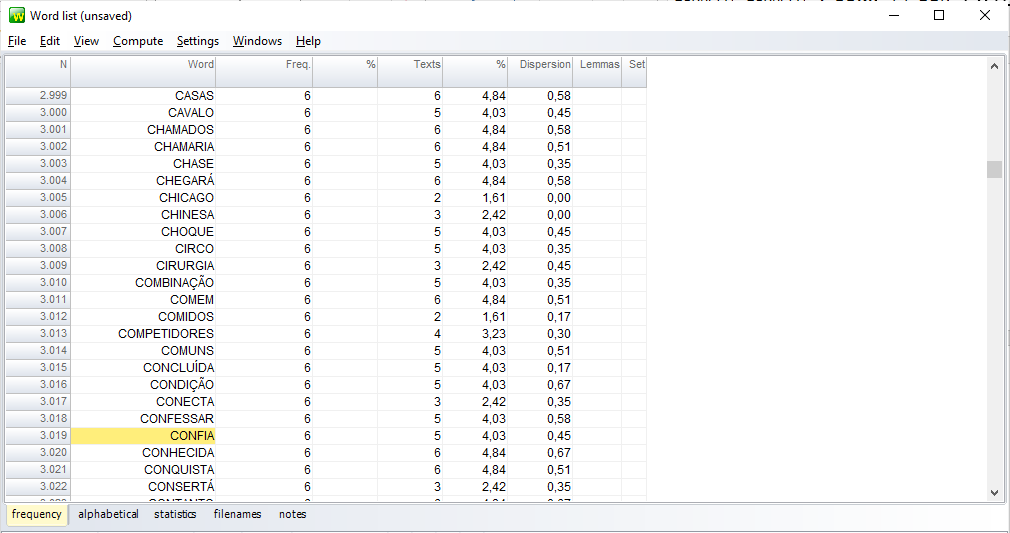
\includegraphics[width=0.85\textwidth]{Fig33.png}
 \caption{Lista de palavras após ser criada.}
 \label{fig33}
 \source{Elaboração nossa.}
\end{figure}

\section{Apresentando e discutindo os resultados do CorLeAni}\label{sec-resumo}
Concluídas as principais fases das pesquisas, descritas na \Cref{sec-conduta}, voltamos os nossos olhares para os dados estatísticos obtidos. Para tanto, exibimos os gráficos nas \Cref{fig34} e \Cref{fig35}, em que, no primeiro, comparamos os \textit{types} e os \textit{tokens}, e, no segundo, o \textit{TTR (Type/Token Ratio)} e \textit{STTR (Standardized Type/Token Ratio)}.

\begin{figure}[htbp]
 \centering
 \begin{minipage}{.45\textwidth}
 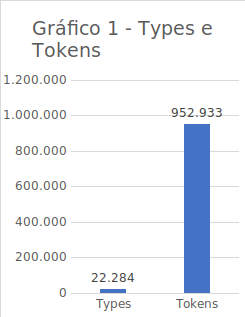
\includegraphics[width=0.9\textwidth]{Fig34.png}
 \caption{Gráfico 1 que mostra os resultados gerais do CorLeAni das pesquisas.}
 \label{fig34}
 \source{Elaboração nossa.}
 \end{minipage}%
 \qquad
 \begin{minipage}{0.45\textwidth}
 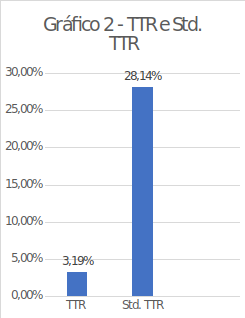
\includegraphics[width=0.9\textwidth]{Graf2.png}
 \caption{Gráfico 2 que mostra os resultados gerais do CorLeAni das pesquisas.}
 \label{fig35}
 \source{Elaboração nossa.} 
 \end{minipage}%
\end{figure}

Na \Cref{fig34}, observamos a quantidade de palavras diferentes no \textit{corpus} (\textit{types}) e palavras gerais (\textit{tokens}), o que indica uma extensão considerável para o CorLeAni, isto é, quase 1 milhão de palavras. Na \Cref{fig35}, apresentamos outros dados em porcentagem, o TTR (\textit{Type/Token ratio}) e \textit{Standardized TTR}, que revelam a variação lexical presente do \textit{corpus}. O primeiro é uma porcentagem de \textit{Types} (palavras diferentes) em relação aos \textit{Tokens} (todas as palavras). O segundo é uma média de porcentagens de \textit{Types} em relação aos \textit{Tokens}, que são feitas a cada 1.000 palavras pelo \textit{WordSmith Tools}.

Um achado interessante que corrobora os dados estatísticos obtidos é a ocorrência de palavras repetidas no \textit{corpus}, como podemos observar na \Cref{fig36}, conforme atestados pelos resultados obtidos por meio da ferramenta \textit{Concord}. 

\begin{figure}[htbp]
 \centering
 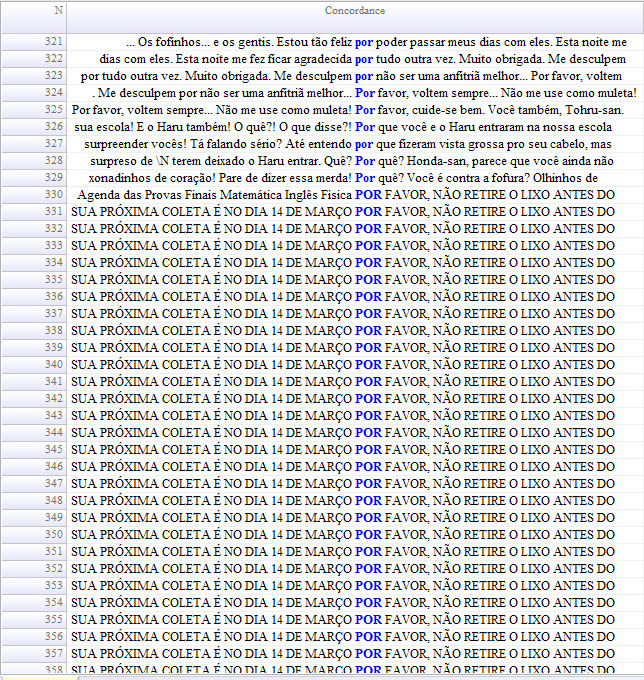
\includegraphics[width=0.85\textwidth]{Fig35.png}
 \caption{Contexto da palavra “por” que aparece diversas vezes no arquivo de legenda, conforme \textit{Concord}, ferramenta do \textit{WordSmith Tools©} (versão 7).}
 \label{fig36}
 \source{Elaboração nossa.}
\end{figure}

Lançamos a hipótese de que essa repetição tenha aparecido nos arquivos de legenda por se tratar da apresentação, na tela, de legendas karaokês ou legendas que estão traduzindo uma parte do cenário, tais como placas, letreiros, entre outras. Trata-se de informações que, ao serem traduzidas, eventualmente demandam a criação de várias linhas de legenda. Para exemplificar tal questão da tradução intersemiótica, podemos pensar em uma cena de uma placa em movimento. Nesse caso, pode-se ter a criação de várias legendas sequenciais e a repetição da mesma frase para tornar a palavra mais visível, de forma que ela apareça na placa mesmo estando em movimento.

Outro achado interessante no \textit{corpus} foi a presença de números e letras individuais utilizados para construir uma frase na vertical, ou, ainda, para realizar algum efeito quando da aparição do vídeo. As \Cref{fig37} e \Cref{fig38} retratam esses resultados.

\begin{figure}[htbp]
 \centering
 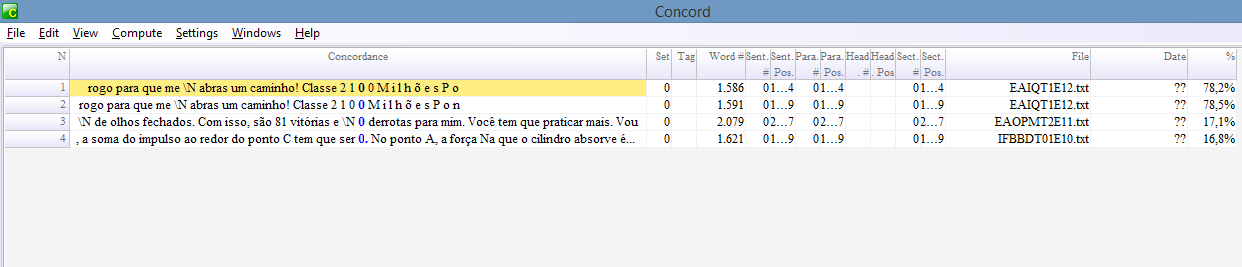
\includegraphics[width=0.85\textwidth]{Fig36.png}
 \caption{Contexto do número 0 no \textit{Concord}.}
 \label{fig37}
 \source{Elaboração nossa.}
\end{figure}

\begin{figure}[h!]
 \centering
 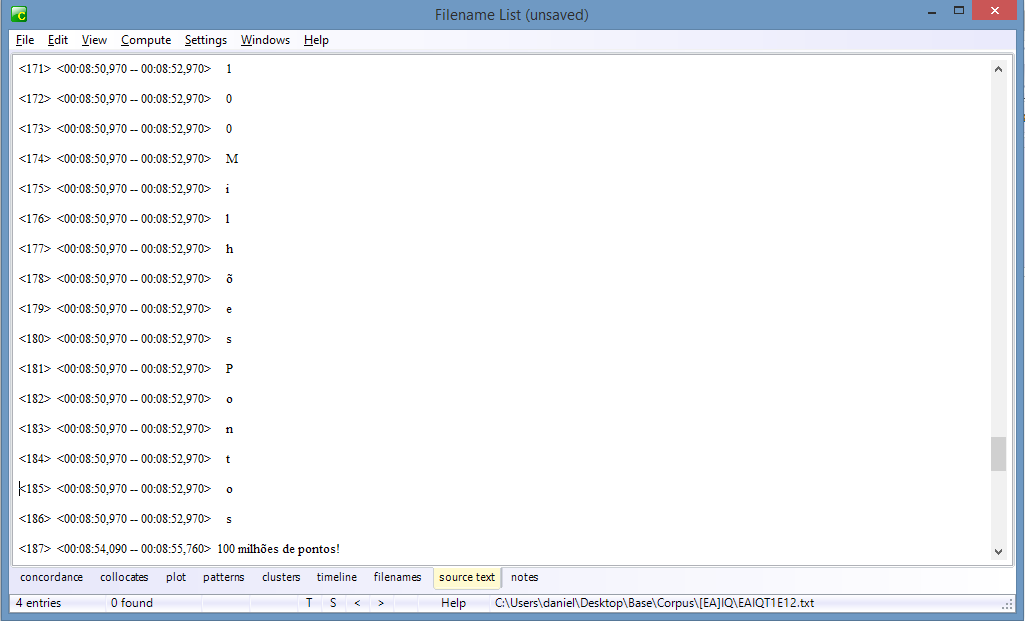
\includegraphics[width=0.85\textwidth]{Fig37.png}
 \caption{Número 0 e outras letras no arquivo de legenda.}
 \label{fig38}
 \source{Elaboração nossa.}
\end{figure}

Para compartilhar os arquivos do CorLeAni e divulgar os resultados das pesquisas, desenvolvemos um \textit{site} que se encontra atualmente hospedado em um domínio grátis na web. Deixamos disponíveis, ademais, um \textit{link} de acesso que redireciona a um serviço de armazenamento da \textit{Microsoft}, o \textit{OneDrive}, e ao serviço de armazenamento da \textit{Google}, o \textit{Google Drive}. O intuito é o de manter possível a realização do \textit{download} de todo material compilado.

\section{Considerações finais}\label{sec-secoes}
Neste artigo, tivemos como objetivo reportar os resultados de dois projetos de iniciação científica que resultaram na compilação do CorLeAni. De acordo com \textcite[p. 1]{diaz-cintas_fansubs:_2006}, “não seria exagero afirmar que as \textit{fansubs} são a manifestação mais importante da tradução de legendas feita por fãs”\footnote{“\textit{It would be no exaggeration to state that fansubs are nowadays the most important manifestation of fan translation} [...]” \cite[p. 1, tradução nossa]{diaz-cintas_fansubs:_2006}.}. Como forma de alavancar esses estudos, reconhecemos o valor que as \textit{fansubs} têm a agregar às discussões e aos estudos no âmbito audiovisual e \textit{fandom}. 

Até o fim do desenvolvimento das pesquisas, o CorLeAni contava com cerca de 1 milhão de palavras, número bastante representativo para servir a futuras investigações no âmbito da tradução e linguagens. Contudo, é importante apontarmos que, durante a execução dos projetos, enfrentamos diversos desafios. Um deles foi a quantidade de legendas selecionadas pelos critérios, um total de 181 arquivos de legendas (PIBIC 2019-2020) e 136 arquivos de legendas (PIBIC 2020-2021), para diferentes obras e legendadas por grupos distintos de \textit{fansubbers}. Esse fato fez com que o tempo demandado na etapa de coleta de dados e edição das legendas fosse maior do que o esperado.

A grande quantidade de linhas de legendas com a mesma frase ou com apenas uma letra nos arquivos de legenda foi, para nós, um grande impasse. Contudo, nos foi possível refletir em torno de perguntas como “O que é uma \textit{fansub}?”, “O que caracteriza uma \textit{fansub}?”. As questões nos levaram a utilizar, como principal referencial teórico, o artigo de \textcite{diaz-cintas_fansubs:_2006}. A partir da leitura do texto, conseguimos chegar ao entendimento de que essas peculiaridades são parte das legendas dos fãs, e retirá-las ou desconsiderá-las da composição do \textit{corpus} seria o mesmo que descaracterizá-las. Com isso em mente, preferimos criar etiquetas nos cabeçalhos das legendas, indicando as partes em que esses casos eram notados.

No entanto, para as informações que não são exibidas ao público, não conseguimos ter o mesmo entendimento das duplicações nas linhas de legendas, pois, em alguns momentos, foi possível constatar a presença de \textit{links} de \textit{sites} de pesquisa. Assim, resolvemos colocá-los entre angulares ( < > ) de forma a não serem contabilizados pelo \textit{WordList}. Contudo, alguns exemplares permanecerem nos arquivos de legendas. Isso não impede, todavia, a possibilidade de serem utilizados em futuros estudos sobre \textit{fansubs}.

Os códigos de formatação e a repetição de frases nas linhas dos arquivos de legenda foi algo que nos trouxe um grande impasse, acarretando uma demanda maior de tempo na etapa de edição de legendas, potencializada principalmente pela quantidade de arquivos a serem editados. Após um estudo teórico e de possíveis ferramentas, tomamos as decisões que foram relatadas anteriormente neste artigo na \Cref{sec-autores}, que, para o caso dos códigos de formatação, foi utilizar a ferramenta “\textit{conversão em lote}”.

Destacamos ainda que a quantidade de palavras (+255.287 \textit{tokens}) inseridas na versão do \textit{corpus} do PIBIC-EM 2020-2021 foi menor em comparação com o PIBIC-EM 2019-2020 (697.646 \textit{tokens}). Atualmente, o CorLeAni em si tornou-se maior e mais representativo do que a sua versão anterior, no sentido da consolidação do \textit{corpus} por meio da adição de mais palavras, advindas de legendas de novos \textit{animes} de gêneros diversos (ação, comédia, romance, entre outros) e do lançamento de novas temporadas. Apesar de o conceito representatividade ser um ponto sobre o qual parece não haver muito consenso dentro da LC \cite{sardinha_linguistica_2004}, reiteramos que, para os objetivos das nossas pesquisas, o \textit{corpus}, em sua atual versão, configura-se como representativo da população de \textit{animes} que gostaríamos de retratar, ilustrados pelas seções das \Cref{sec-conduta} e \Cref{sec-resumo}.

Como pesquisadores, as problemáticas que nos foram apresentadas em ambos os projetos nos fascinaram e nos motivaram a seguir com o nosso trabalho. Hoje, após dois anos de pesquisas, percebemos que ainda há muito para se estudar e explorar sobre temas relacionados às \textit{fansubs}. Concluímos as investigações com um sentimento de satisfação, por termos contribuído com algo que tem a sua relevância nas discussões e estudos no âmbito audiovisual. Atribuímos uma ênfase também no ato de legendar, observando como as \textit{fansubs} fazem uso do karaokê, de notas explicativas e que mantêm, às vezes, os honoríficos (sufixos como \textit{-Kun} ou \textit{-sensei}, utilizados no Japão para demonstrar uma distância social), além de outras particularidades.

Ademais, ponderamos que outros pesquisadores podem realizar o download dos arquivos de ambos os projetos e alterar os dados ou arquivos de legendas para atender aos seus objetivos e particularidades de cada pesquisa. A riqueza de dados disponível no \textit{corpus} pode iluminar pesquisas que analisem variados aspectos linguísticos e tradutórios, como é o caso, por exemplo, do estilo das \textit{fansubs}, as suas palavras específicas, os comentários dos tradutores como paratextos que não são exibidos para o espectador, mas que trazem indícios de autoria, entre outros aspectos.

A pandemia da COVID-19 foi algo que também impactou as pesquisas, particularmente o desenvolvimento do projeto PIBIC-EM 2020-2021, por impedir encontros e debates de forma presencial com o orientador e a comunidade acadêmica. Para resolver essa questão, utilizamos inicialmente o \textit{Skype}, que permite a realização de videochamada e ligações por voz e, em seguida, a plataforma \textit{Google Meet}. Em suma, conseguimos solucionar os problemas e dar sequência à execução dos projetos sem mais complicações. 

Por fim, avaliamos que a experiência de desenvolver as pesquisas por meio do Programa de Iniciação Científica, via concessão de bolsas PIBIC-EM/IF Goiano, foi bastante enriquecedora em várias frentes, tanto para o aluno-bolsista, quanto para o orientador. Observamos de imediato a importância da pesquisa júnior já no âmbito da educação básica, profissional e tecnológica, no sentido de despertar a vocação científica, servindo como importante forma de incentivar talentos entre estudantes com excelência acadêmica. A partir dos dois projetos desenvolvidos, foi possível, especialmente por parte do aluno-bolsista, debruçar-se sobre uma nova área de conhecimento, os seus principais autores e as teses por eles defendidas; aprender sobre metodologia científica; defrontar-se com os problemas reais de se desenvolver pesquisa e ainda assim propor soluções que levaram, de forma organizada e criteriosa, ao resultado final almejado pelos projetos. Assim sendo, almejamos que o \textit{corpus} possa ser de grande auxílio à comunidade acadêmica e iluminar futuras pesquisas.

\section{Agradecimento}
Agradecemos ao Programa de Iniciação Científica do Instituto Federal de Educação, Ciência e Tecnologia Goiano a concessão de bolsas PIBIC-EM/IF Goiano para realização desta pesquisa.

\printbibliography\label{sec-bib}
% if the text is not in Portuguese, it might be necessary to use the code below instead to print the correct ABNT abbreviations [s.n.], [s.l.]
%\begin{portuguese}
%\printbibliography[title={Bibliography}]
%\end{portuguese}


%full list: conceptualization,datacuration,formalanalysis,funding,investigation,methodology,projadm,resources,software,supervision,validation,visualization,writing,review
\begin{contributors}[sec-contributors]
\authorcontribution{Daniel Gomes da Cunha}[datacuration,formalanalysis,investigation,methodology,software,validation,visualization,writing,review]
\authorcontribution{Janailton Mick Vitor da Silva}[conceptualization,funding,methodology,projadm,resources,supervision,validation,review]
\end{contributors}

\end{document}
